\documentclass[12pt,a4wide]{report}

\usepackage{amsthm,amssymb,mathrsfs,setspace}
\usepackage[nottoc]{tocbibind}
\renewcommand{\chaptermark}[1]{\markboth{#1}{}}
\renewcommand{\sectionmark}[1]{\markright{\thesection\ #1}}

\usepackage{graphicx}
\usepackage{adjustbox}
\usepackage{amsmath}
\usepackage{pgfplots}
\pgfplotsset{compat=1.18}
\usepackage{hyperref}
\usepackage{xcolor}
\usepackage{booktabs}
\usepackage{array}
\usepackage{enumitem}
\usepackage{fancyhdr}
\usepackage{setspace}
\usepackage{listings}
\usepackage{float}
\usepackage{multirow}
\usepackage{makecell}
\usepackage[T1]{fontenc}
\usepackage[utf8]{inputenc}
\usepackage{microtype}
\usepackage{geometry}
\geometry{a4paper, left=3.5cm, right=2.5cm, top=2.5cm, bottom=2.5cm}

% ── TikZ for all diagrams ─────────────────────────────────────────────────────

\usepackage{tikz}
\usetikzlibrary{shapes.geometric, shapes.misc, arrows.meta, positioning,
                fit, backgrounds, shadows, calc, decorations.pathreplacing,
                patterns, matrix,calc}

\definecolor{primaryblue}{RGB}{26,86,159}
\definecolor{accentgreen}{RGB}{0,128,80}
\definecolor{darkgray}{RGB}{60,60,60}
\definecolor{codebg}{RGB}{250,250,250}
\definecolor{borderblue}{RGB}{100,149,237}

\hypersetup{
  colorlinks=true,
  linkcolor=primaryblue,
  citecolor=accentgreen,
  urlcolor=primaryblue,
  pdftitle={A Blockchain Based Decentralised Health Record System},
  pdfauthor={Shashank Upadhyay, Anushila Biswas, Vyshnavi Reddy Battula, Suraj Rathor}
}

\lstset{
  backgroundcolor=\color{codebg},
  basicstyle=\ttfamily\small,
  breaklines=true,
  frame=single,
  rulecolor=\color{borderblue},
  keywordstyle=\color{primaryblue}\bfseries,
  commentstyle=\color{accentgreen}\itshape,
  stringstyle=\color{red},
  numbers=left,
  numberstyle=\tiny\color{darkgray},
  stepnumber=1,
  numbersep=8pt,
  captionpos=b
}

\tikzset{
  layerbox/.style={
    draw=#1!70!black, fill=#1!18, rounded corners=6pt,
    minimum width=3.2cm, minimum height=1.0cm,
    font=\small\bfseries, text=#1!60!black, align=center,
    drop shadow={shadow xshift=1.5pt, shadow yshift=-1.5pt, opacity=0.18}
  },
  actor/.style={
    draw=primaryblue!70, fill=lightblue, rounded corners=4pt,
    minimum width=2.6cm, minimum height=0.85cm,
    font=\small\bfseries, text=primaryblue!80, align=center
  },
  usecase/.style={
    draw=accentgreen!70, fill=lightgreen, ellipse,
    minimum width=3.4cm, minimum height=0.75cm,
    font=\scriptsize, text=accentgreen!80, align=center
  },
  seqbox/.style={
    draw=#1!70!black, fill=#1!15, rounded corners=4pt,
    minimum width=2.0cm, minimum height=0.7cm,
    font=\scriptsize\bfseries, text=#1!80!black, align=center
  },
  seqline/.style={draw=darkgray!50, thick},
  msgarrow/.style={-Stealth, draw=primaryblue!80, thick},
  retarrow/.style={-Stealth, draw=darkgray!60, dashed, thick},
  encbox/.style={
    draw=#1!70!black, fill=#1!15, rounded corners=5pt,
    minimum width=2.4cm, minimum height=0.75cm,
    font=\scriptsize\bfseries, text=#1!80!black, align=center
  },
  secring/.style={
    draw=#1!70!black, fill=#1!12, rounded corners=8pt,
    font=\scriptsize\bfseries, text=#1!80!black, align=center
  }
}

\newcommand{\ArchitectureDiagram}[1]{%
\resizebox{#1\textwidth}{!}{%
\begin{tikzpicture}[
    node distance=1.5cm and 1cm,
    % FIXED: Changed #1 to ##1 to prevent macro argument clashing
    layerBox/.style={rectangle, draw=##1!80, fill=##1!10, dashed, thick, rounded corners=15pt, inner sep=15pt},
    appNode/.style={rectangle, draw=cyan!80!blue, fill=cyan!15, rounded corners=5pt, minimum width=3cm, minimum height=1.2cm, align=center, font=\small\bfseries, text=black!80},
    apiNode/.style={rectangle, draw=orange!80!red, fill=orange!15, rounded corners=5pt, minimum width=4cm, minimum height=1.2cm, align=center, font=\small\bfseries, text=black!80},
    scNode/.style={rectangle, draw=green!70!black, fill=green!15, rounded corners=5pt, minimum width=4cm, minimum height=1.2cm, align=center, font=\small\bfseries, text=black!80},
    storeNode/.style={rectangle, draw=purple!70, fill=purple!15, rounded corners=5pt, minimum width=4cm, minimum height=1.2cm, align=center, font=\small\bfseries, text=black!80},
    layerTitle/.style={font=\Large\bfseries, anchor=south west},
    layerSub/.style={font=\footnotesize, text=gray!80!black, anchor=north west},
    solidArrow/.style={-{Stealth[scale=1.2]}, thick, draw=gray!90!black},
    dashedArrow/.style={-{Stealth[scale=1.2]}, thick, dashed, draw=gray!90!black}
]

% ================= APPLICATION LAYER =================
\node[appNode] (doctor) {Doctor\\Dashboard};
\node[appNode, right=0.6cm of doctor] (patient) {Patient\\Dashboard};
\node[appNode, right=0.6cm of patient] (delegate) {Delegate\\View};
\node[appNode, right=0.6cm of delegate] (admin) {Admin\\Panel};

\node[layerTitle, text=cyan!80!blue] (appTitle) at ([yshift=1cm, xshift=-0.5cm]doctor.north west) {Application Layer};
\node[layerSub] (appSub) at ([yshift=-0.1cm]appTitle.south west) {React, Vite, Tailwind CSS, MetaMask (Wallet)};

\begin{scope}[on background layer]
    \node[layerBox=cyan, fit=(doctor) (patient) (delegate) (admin) (appTitle) (appSub)] (appLayer) {};
\end{scope}

% ================= BACKEND LAYER =================
\node[apiNode, below=3.5cm of doctor, xshift=1.5cm] (api) {REST API\\(Express.js)};
\node[apiNode, right=1cm of api] (queue) {Request Queue\\\& Metadata};

\node[layerTitle, text=orange!80!red] (apiTitle) at ([yshift=1cm, xshift=-0.5cm]api.north west) {Backend Services Layer};
\node[layerSub] (apiSub) at ([yshift=-0.1cm]apiTitle.south west) {Node.js, Authentication, Payload Routing};

\begin{scope}[on background layer]
    \node[layerBox=orange, fit=(api) (queue) (apiTitle) (apiSub)] (apiLayer) {};
\end{scope}

% ================= SMART CONTRACT LAYER =================
\node[scNode, below=3.5cm of api] (registry) {Prescription Registry};
\node[scNode, below=3.5cm of queue] (oracle) {DoctorStatus Oracle};

\node[layerTitle, text=green!70!black] (scTitle) at ([yshift=1cm, xshift=-0.5cm]registry.north west) {Smart Contract Layer};
\node[layerSub] (scSub) at ([yshift=-0.1cm]scTitle.south west) {Polygon PoS, EVM, Solidity 0.8.23};

\begin{scope}[on background layer]
    \node[layerBox=green, fit=(registry) (oracle) (scTitle) (scSub)] (scLayer) {};
\end{scope}

% ================= STORAGE LAYER =================
\node[storeNode, right=2.5cm of queue, yshift=-0.5cm] (ipfs) {IPFS Network\\(Encrypted Bundles)};
\node[storeNode, below=1.5cm of ipfs] (pinata) {Pinata\\(Cloud Pinning)};

\node[layerTitle, text=purple!80!black] (storeTitle) at ([yshift=1cm, xshift=-0.5cm]ipfs.north west) {Storage Layer};
\node[layerSub] (storeSub) at ([yshift=-0.1cm]storeTitle.south west) {Content-Addressed Off-Chain};

\begin{scope}[on background layer]
    \node[layerBox=purple, fit=(ipfs) (pinata) (storeTitle) (storeSub)] (storeLayer) {};
\end{scope}

% ================= INTER-LAYER ARROWS =================
\draw[solidArrow] (apiLayer.north |- appLayer.south) -- node[right, font=\footnotesize, text=gray] {API calls} (apiLayer.north);
\draw[solidArrow] (scLayer.north |- apiLayer.south) -- node[right, font=\footnotesize, text=gray] {tx / view} (scLayer.north);
\draw[solidArrow] (apiLayer.east) -- node[above, font=\footnotesize, text=gray] {pin / fetch} (apiLayer.east -| storeLayer.west);
\draw[dashedArrow] (scLayer.east) -- node[above, font=\footnotesize, text=gray] {CID anchor} (scLayer.east -| storeLayer.west);
\draw[dashedArrow] (appLayer.south -| admin.south) -- node[right, font=\footnotesize, text=gray] {CID fetch} (storeLayer.north -| admin.south);

% ================= LEGEND =================
\node[anchor=west, font=\footnotesize\color{gray}] (legend1text) at ([yshift=-1.5cm, xshift=1cm]scLayer.south west) {Direct call / transaction};
\draw[solidArrow] ([xshift=-1.5cm]legend1text.west) -- ([xshift=-0.2cm]legend1text.west);

\node[anchor=west, font=\footnotesize\color{gray}] (legend2text) at ([xshift=4cm]legend1text.east) {Content addressing / browser-side};
\draw[dashedArrow] ([xshift=-1.5cm]legend2text.west) -- ([xshift=-0.2cm]legend2text.west);

\end{tikzpicture}%
}%
}

\newcommand{\WorkflowDiagram}[1]{%
\begin{tikzpicture}[font=\sffamily\scriptsize, scale=#1, every node/.style={transform shape}]
  \tikzset{
    lane/.style={rectangle, rounded corners=4pt, minimum width=2.0cm, minimum height=0.6cm, align=center, thick, draw=gray!55, fill=white, drop shadow={opacity=0.12}},
    msg/.style={-{Stealth[length=2.7mm]}, thick},
    guide/.style={dashed, draw=gray!55}
  }

  \node[lane, fill=green!10, draw=green!50] (d) at (0,0) {\textbf{Doctor}};
  \node[lane, fill=cyan!10, draw=cyan!55] (b) at (3.6,0) {\textbf{Backend/IPFS}};
  \node[lane, fill=blue!10, draw=blue!55] (p) at (7.2,0) {\textbf{Patient}};
  \node[lane, fill=purple!10, draw=purple!55] (r) at (10.8,0) {\textbf{Registry}};

  \foreach \x in {0,3.6,7.2,10.8} {
    \draw[guide] (\x,-0.35) -- (\x,-6.6);
  }

  \draw[msg, draw=green!60!black] (0,-0.9) -- node[above, align=center] {1. encrypt + sign\\ request} (3.6,-0.9);
  \draw[msg, draw=cyan!65!black] (3.6,-1.8) -- node[above] {2. request available} (7.2,-1.8);
  \draw[msg, draw=blue!65!black] (7.2,-2.7) -- node[above] {3. fetch encrypted bundle} (3.6,-2.7);
  \draw[msg, draw=blue!65!black] (7.2,-3.6) -- node[above, align=center] {4. patient signs\\ approval} (10.8,-3.6);
  \draw[msg, draw=purple!65!black] (7.2,-4.5) -- node[above, align=center] {5. \texttt{registerPrescription()}} (10.8,-4.5);
  \draw[msg, draw=purple!65!black, dashed] (10.8,-5.3) -- node[above] {6. \texttt{PrescriptionIssued}} (7.2,-5.3);
  \draw[msg, draw=blue!65!black] (7.2,-6.1) -- node[above, align=center] {7. store tx hash\\ + id} (3.6,-6.1);
\end{tikzpicture}%
}

\newcommand{\IntegrityDiagram}[1]{%
\begin{tikzpicture}[font=\sffamily, scale=#1, every node/.style={transform shape}]
  \tikzset{
    box/.style={rectangle, rounded corners=5pt, minimum width=2.6cm, minimum height=0.8cm, align=center, thick, draw=gray!55, fill=white, drop shadow={opacity=0.12}},
    flow/.style={-{Stealth[length=3mm]}, thick, draw=gray!75},
    warn/.style={rectangle, rounded corners=5pt, minimum width=2.8cm, minimum height=0.8cm, text width=2.45cm, align=center, thick, draw=red!60, fill=red!5}
  }

  \node[box, fill=green!8, draw=green!45] (record) at (0,1.8) {\textbf{Encrypted Record}};
  \node[box, fill=blue!8, draw=blue!45] (hash) at (3.3,1.8) {\textbf{Content Hash}};
  \node[box, fill=orange!8, draw=orange!50] (cid) at (6.6,1.8) {\textbf{CID}};
  \node[box, fill=purple!8, draw=purple!55] (block) at (9.9,1.8) {\textbf{Block Anchor}};

  \draw[flow] (record) -- (hash);
  \draw[flow] (hash) -- (cid);
  \draw[flow] (cid) -- (block);

  \node[warn] (tamper) at (3.3,0.1) {\textbf{Record modified}};
  \node[warn] (newhash) at (6.6,0.1) {\textbf{Hash/CID}\\\textbf{changes}};
  \node[warn] (break) at (9.9,0.1) {\textbf{Old block no}\\\textbf{longer matches}};

  \draw[flow, draw=red!70] (tamper) -- (newhash);
  \draw[flow, draw=red!70] (newhash) -- (break);

  \node[box, fill=purple!8, draw=purple!55, minimum width=3.4cm] (next) at (13.5,1.8) {\textbf{Next Block}\\ \tiny stores previousHash};
  \draw[flow] (block) -- (next);
  \node[warn, minimum width=3.4cm, text width=3.0cm] (chainbreak) at (13.5,0.1) {\textbf{Downstream}\\\textbf{validation fails}};
  \draw[flow, draw=red!70] (break) -- (chainbreak);
\end{tikzpicture}%
}


\renewcommand{\baselinestretch}{1.5}

% ══════════════════════════════════════════════════════════════════════════════
\begin{document}

% ── Title Page ────────────────────────────────────────────────────────────────
\begin{titlepage}
\enlargethispage{1cm}
\begin{center}

\vspace*{-1.2cm}

{\bfseries\Large A BLOCKCHAIN BASED DECENTRALISED HEALTH RECORD SYSTEM}\\[8pt]

\vspace*{1.0cm}

A Project Report Submitted \\
in Partial Fulfilment of the Requirements \\
for the Degree of \\
\vspace{3mm}
{\Large \bf BACHELOR OF TECHNOLOGY} \\
\vspace{4mm}
in \\
\vspace{2mm}
{\large \bf COMPUTER SCIENCE AND ENGINEERING} \\

\vspace{6mm}
{\em by}\\[3mm]
\begin{tabular}{cc}
\textbf{Shashank Upadhyay} & \textbf{Anushila Biswas} \\
(2022BCS0088) & (2022BCS0069) \\[2mm]
\textbf{Vyshnavi Reddy Battula} & \textbf{Suraj Rathor} \\
(2022BCS0133) & (2022BCS0051)
\end{tabular}\\[6mm]
Under the Supervision of \\
{\large \bf Dr.\ Anu Maria Sebastian} \\

\vspace{8mm}

\includegraphics[width=4.8cm,height=2.4cm,keepaspectratio]{logo2.jpg}\\[4mm]
{\bf \mbox{DEPARTMENT OF COMPUTER SCIENCE AND ENGINEERING}} \\
{\bf \mbox{INDIAN INSTITUTE OF INFORMATION TECHNOLOGY}}\\
{\bf KOTTAYAM-686635, INDIA}\\[2mm]
{\it April 2026}

\end{center}
\end{titlepage}

\clearpage
% --------------- Declaration  page -----------------------
\pagenumbering{roman} \setcounter{page}{2}
\begin{center}
{\large{\bf{DECLARATION}}}
\end{center}

\noindent We, \textbf{Shashank Upadhyay (2022BCS0088), Anushila Biswas (2022BCS0069), Vyshnavi Reddy Battula (2022BCS0133), and Suraj Rathor (2022BCS0051)}, hereby declare that this report entitled \textbf{``A Blockchain Based Decentralised Health Record System''} submitted to Indian Institute of Information Technology Kottayam towards partial requirement of {\bf Bachelor of Technology} in \textbf{Computer Science and Engineering} is an original work carried out by us under the supervision of \textbf{Dr.\ Anu Maria Sebastian} and has not formed the basis for the award of any degree or diploma, in this or any other institution or university. We have sincerely tried to uphold academic ethics and honesty. Whenever external information, statements, or results are used, they have been duly acknowledged and cited.

\vspace{4cm}

\noindent Kottayam-686635 \hfill \textbf{Shashank Upadhyay (2022BCS0088)}

\noindent April 2026 \hfill \textbf{Anushila Biswas (2022BCS0069)}

\hfill \textbf{Vyshnavi Reddy Battula (2022BCS0133)}

\hfill \textbf{Suraj Rathor (2022BCS0051)}

\clearpage

% --------------- Certificate page -----------------------
\pagenumbering{roman} \setcounter{page}{3}
\begin{center}
{\large{\bf{CERTIFICATE}}}
\end{center}

\noindent This is to certify that the work contained in this project report entitled \textbf{``A Blockchain Based Decentralised Health Record System''} submitted by \textbf{Shashank Upadhyay (2022BCS0088), Anushila Biswas (2022BCS0069), Vyshnavi Reddy Battula (2022BCS0133), and Suraj Rathor (2022BCS0051)} to the Indian Institute of Information Technology Kottayam towards partial requirement of {\bf Bachelor of Technology} in \textbf{Computer Science and Engineering} has been carried out under my supervision and that it has not been submitted elsewhere for the award of any degree.

\vspace{4cm}

\noindent Kottayam-686635 \hfill \textbf{(Dr.\ Anu Maria Sebastian)}

\noindent April 2026 \hfill Project Supervisor\\

\vspace{2.5cm}
\noindent\hfill\hfill \textbf{(Dr.\ Christina Terese Joseph)}

\noindent \hfill Head of the Department

\noindent\hfill\hfill Dept. of Computer Science \& Engineering\\

\clearpage

% ── Acknowledgement ───────────────────────────────────────────────────────────
\begin{center}
{\Large{\bf{ACKNOWLEDGEMENT}}}
\end{center}
\addcontentsline{toc}{chapter}{Acknowledgement}

We would like to express our sincere gratitude to \textbf{Dr.\ Anu Maria Sebastian}
for her constant guidance, encouragement, and constructive feedback throughout the
course of this project. Her support helped us refine both the technical direction
and the academic presentation of this work.

We are also thankful to the \textbf{Department of Computer Science and Engineering,
Indian Institute of Information Technology Kottayam}, for providing the academic
environment, infrastructure, and resources necessary to carry out this project.

We extend our gratitude to our faculty members, classmates, and peers for their
valuable suggestions and discussions during the development and evaluation phases.
Their inputs were helpful in improving the implementation, testing strategy, and
overall clarity of the system.

Finally, we thank our families and well-wishers for their continuous encouragement,
patience, and support throughout the duration of this work.

\clearpage

% ── Abstract ──────────────────────────────────────────────────────────────────
\begin{center}
{\Large{\bf{ABSTRACT}}}
\end{center}
\addcontentsline{toc}{chapter}{Abstract}

This is a blockchain based prescription registry designed to enable dual-signature validation and patient-controlled access to electronic medical records. Conventional Electronic Health Record (EHR) systems rely on centralised infrastructures, which often result in fragmented interoperability, increased vulnerability to data breaches, and limited patient control over sensitive health information.

To address these limitations, it integrates three core technologies: the Polygon Layer-2 blockchain for scalable and tamper-resistant transaction management, the InterPlanetary File System (IPFS) for secure off-chain storage of encrypted medical data, and Solidity-based smart contracts to enforce decentralised and fine-grained access control. The system ensures that prescriptions are validated through a dual-signature EIP-712 protocol, requiring independent approval from both the physician and the patient before being committed on-chain.

Security is further enhanced through end-to-end AES-256-GCM encryption and a hybrid key management approach, ensuring that sensitive data remains protected and inaccessible to unauthorised entities. Additional mechanisms include decentralised physician verification and automated re-encryption to support secure delegation of access without repeated patient intervention.

To evaluate system performance and security, a suite of tools was developed, including contract-only blockchain tests, a synthetic dataset generator, a local-chain load benchmark, a blockchain tamper simulation, and a workload projection model. The current prototype baseline records draft creation at 13.38~s, finalisation at 12.79~s, delegate approval at 7.99~s, Pinata upload at 1.28~s mean, and API latency at 19.95~ms mean under local test conditions. Security analysis confirms resilience against unauthorised access, replay attempts, and data tampering while the contract test suite passes in full.

Overall, This system provides a secure, scalable, and patient-centric alternative to traditional EHR systems, improving data ownership, interoperability, and trust in healthcare data management.

\tableofcontents
\listoffigures
\listoftables

% ══════════════════════════════════════════════════════════════════════════════
\chapter{Introduction}
% ══════════════════════════════════════════════════════════════════════════════

\section{Background}

Electronic Health Record (EHR) systems are digital platforms designed to capture,
store, and manage patient medical information across the continuum of care. By
enabling healthcare practitioners to retrieve, exchange, and update clinical data
in a structured and consistent manner, EHR systems have significantly improved
coordination within individual healthcare institutions. Historically, however,
these systems have been built on centralised server infrastructure managed by
a single hospital, clinic, or government health authority a design choice that
was natural at the time of their creation but which carries increasingly serious
consequences as healthcare becomes more distributed and adversarial threats more
sophisticated.

The centralised EHR model introduces three structural weaknesses that this project
directly targets. First, \textit{data siloing}: each institution operates its own
isolated repository using proprietary data formats and schemas. When a patient
moves between providers visiting a specialist, transferring to a different
hospital, or relocating to another city their medical history does not travel
with them. Clinicians are forced to make decisions with incomplete information,
patients undergo redundant diagnostic tests, and the healthcare system bears
unnecessary costs. Second, \textit{concentrated attack surface}: all of an
organisation's patient records reside in a single system, making that system an
extremely high-value target for ransomware operators and data thieves. A single
successful breach can expose hundreds of thousands of detailed personal profiles
simultaneously. Healthcare data commands premium prices on criminal markets because
it combines demographic, financial, and sensitive biological information in one
profile. Third, \textit{absent patient control}: patients typically have no
practical mechanism to audit who has accessed their records, for what purpose, or
under what authority. They cannot selectively share specific records with a new
provider or revoke access once granted. This asymmetry fundamentally undermines
the ethical principle of patient autonomy.

\section{Motivation and Problem Statement}

The growing digitisation of healthcare and the expanding adoption of telemedicine,
wearable monitoring, and cross-border medical tourism have made the interoperability
failures of centralised EHR systems increasingly acute. At the same time, regulatory
frameworks such as HIPAA in the United States and GDPR in the European Union now
impose strict requirements on consent management, data access logging, and the
right to data portability requirements that centralised systems satisfy imperfectly
at best.

Blockchain technology offers a fundamentally different architectural starting point.
A blockchain is a distributed ledger in which records are cryptographically chained
so that any retroactive modification is computationally infeasible without
controlling a majority of the network. No single party owns or controls the ledger;
every participant maintains a consistent copy. Smart contracts programs deployed
and executed on the blockchain allow complex access-control logic and business
workflows to be automated without requiring a trusted intermediary. These properties
collectively address the three structural weaknesses of centralised EHR: a shared
ledger eliminates siloing, distribution eliminates the single point of failure, and
smart contracts give patients programmable, cryptographically enforced control over
their data.

The proposed blockchain based health record system was conceived to demonstrate that these theoretical properties can be
realised in a working, evaluable system with performance characteristics compatible
with real clinical workflows.

\section{Proposed System}

The proposed system adopts a \textbf{hybrid architecture} that separates the concerns of
trust and storage. Encrypted medical documents are stored off-chain on IPFS
a distributed content-addressed storage network while the Polygon blockchain
retains only the cryptographic Content Identifiers (CIDs) that reference them.
This separation keeps the blockchain lean and economically viable while still
providing an immutable, tamper evident reference to every medical record. Smart
contracts deployed on Polygon govern every access decision: who may create a
prescription, who may read it, who may delegate access to a third party, and how
any of these permissions may be revoked.

The system was developed across three formal review cycles. The first cycle
established the core dual-signature prescription workflow. The second added
IPFS-backed storage, patient delegation, and the React/MetaMask frontend. The
third the final cycle described in this report introduced end-to-end
AES-256-GCM encryption with hybrid key derivation, the DoctorStatusOracle
contract, automated re-encryption upon delegation, and a full suite of evaluation
tooling. By the final review the system had matured from a functional prototype
into a security hardened research prototype with a reproducible evaluation package.

\section{System Overview}

The platform is organised across four interdependent layers:

\begin{itemize}
  \item \textbf{Blockchain Layer:} Polygon (Ethereum Layer-2, Proof-of-Stake)
    records all prescription lifecycle events, hosts both smart contracts, and
    maintains a tamper proof audit trail that any authorised party can inspect.
    Polygon's PoS consensus delivers sub-two-second transaction finality at gas
    costs orders of magnitude below the Ethereum mainnet.
  \item \textbf{Storage Layer:} IPFS via the Pinata cloud pinning service stores
    encrypted medical documents off-chain. Each file is identified by a
    deterministic CID computed from its content, so any modification however
    minor changes the CID and is immediately detectable. Only CIDs are written
    on-chain, preventing blockchain storage congestion.
  \item \textbf{Application Layer:} A React + Vite + Tailwind CSS frontend
    provides role-specific dashboards for doctors, patients, delegates, and
    administrators. MetaMask, integrated via the Wagmi library, handles wallet
    authentication and transaction signing entirely within the user's browser
    without exposing private keys to any server.
  \item \textbf{Backend Services:} A Node.js / Express.js server orchestrates
    Pinata pinning, manages the prescription request queue, exposes the REST API,
    and serves blockchain-derived metadata to authorised viewers. In the intended
    encrypted workflow, encryption and decryption logic runs in the browser and
    the backend operates primarily on encrypted bundles and metadata; however the
    current prototype still retains compatibility paths for plaintext request
    payloads and is therefore not claimed as a strict zero-knowledge architecture.
\end{itemize}

\section{Objectives}

The specific technical and functional objectives of this project are:

\begin{itemize}
  \item To eliminate dependence on centralised healthcare databases as the sole
    custodians of patient records.
  \item To guarantee the integrity and provenance of every medical record through
    blockchain immutability and cryptographic content addressing.
  \item To protect data confidentiality with AES-256-GCM client-side encryption,
    keeping the main prescription workflow encrypted end-to-end between browser
    and storage while minimizing server side exposure to plaintext medical data.
  \item To implement patient sovereign, smart contract enforced access control
    in which only the patient can authorise or revoke access by third parties.
  \item To enforce dual-signature informed consent at the protocol level, requiring
    cryptographic co-approval from both physician and patient before any prescription
    is permanently committed.
  \item To achieve economic viability through Polygon Layer-2 scaling, making the
    system financially practical for routine clinical prescription volumes.
  \item To deliver an accessible, role-specific web interface suitable for
    real-world healthcare users without deep blockchain expertise.
  \item To provide a rigorous evaluation suite contract tests, prototype
    metrics, local-chain benchmarking, tamper simulation, workload projection,
    and literature comparison grounding all performance and security claims
    in verifiable evidence.
\end{itemize}

\section{Potential Applications}

The proposed system is currently centered on prescriptions, but the same design
pattern extends naturally to several healthcare workflows:

\begin{itemize}
  \item \textbf{Inter-hospital prescription portability:} a patient can carry
    a cryptographically anchored prescription history across providers without
    relying on a single hospital database.
  \item \textbf{Telemedicine and cross-provider consultation:} a doctor can
    issue a digitally signed prescription request remotely, while the patient
    retains explicit approval power before final publication.
  \item \textbf{Specialist referral and delegate access:} a patient can grant
    a new specialist or diagnostic center access to prior records without
    permanently exposing the full record set to all providers.
  \item \textbf{Auditable medical data exchange:} every final publication and
    delegation decision is recorded on-chain, supporting later verification and
    dispute resolution.
\end{itemize}

\section{Scope and Organisation of the Report}

The current version of the proposed system covers the complete prescription lifecycle:
doctor-submitted prescription requests, patient co-signature and on-chain
publication through \texttt{registerPrescription()}, IPFS-backed encrypted
storage, and patient-controlled access delegation with metadata updates for
newly authorised recipients. Full integration with hospital information systems
(HL7/FHIR), support for binary medical imaging formats (DICOM), insurance claim
processing, and emergency access override mechanisms are identified as future
extensions and discussed in Chapter~6.

The remainder of this report is structured as follows. Chapter~2 surveys seven
related systems and presents the literature experiment map. Chapter~3 describes
the methodology and system architecture. Chapter~4 details the implementation of
smart contracts, the encryption scheme, and the deployment workflow. Chapter~5
presents evaluation results from prototype benchmarking, tamper simulation, and
workload projection. Chapter~6 analyses limitations and proposes a future roadmap.
Chapter~7 concludes.

% ══════════════════════════════════════════════════════════════════════════════
\chapter{Literature Review}
% ══════════════════════════════════════════════════════════════════════════════

\section{Overview}

This chapter surveys seven published blockchain-based EHR systems alongside a
structured experiment map generated by the project's \texttt{literature-comparison.js}
tool. The map characterises each paper's experimental design, reported metrics,
and approach to scaling evaluation, enabling an honest positioning of the proposed system's
own evidence without overstating comparability. The chapter concludes with a
gap analysis summarised in Table~\ref{tab:comparison}.

\section{Related Work}

\subsection{Block MedCare - Simonoski and Bogatinoska (2024)}

Simonoski and Bogatinoska present Block MedCare, a decentralised application
(dApp) built on the public Ethereum blockchain using Solidity smart contracts and
a React.js frontend. The system employs Role Based Access Control (RBAC) to govern
the sharing of medical data, and its usability was validated through structured
testing involving practising healthcare professionals. The study's findings
demonstrate genuine clinical interest in blockchain-based interoperability, and
participants responded positively to the transparency properties of the on-chain
access model.

However, Block MedCare is subject to notable limitations. Deployed on the Ethereum
mainnet, it inherits the high per transaction gas costs and variable latency of
Proof-of-Work consensus, making it economically impractical for high volume
prescription management. More critically, the system does not implement end-to-end
encryption data stored on IPFS may be accessible to backend operators and
there is no dual-signature requirement, meaning a prescription can be registered
without the patient's explicit cryptographic consent. The experiment style is a
usability survey combined with a functional prototype, with no throughput or
latency benchmarks.

\subsection{Novel Blockchain EHR - Chelladurai and Pandian (2021)}

Chelladurai and Pandian present an EHR automation platform built on Hyperledger
Fabric, using chaincode (smart contracts) for distributed record management.
A distinctive contribution is the use of a Modified Merkle Tree alongside SHA-256
hashing to construct tamper-evident audit logs. The permissioned nature of Hyperledger
Fabric allows the system to demonstrate meaningfully improved response times and
transaction throughput compared to conventional relational databases. This paper
is the closest available reference for performance style experiments: it reports
CPU utilisation, memory usage, response time, and throughput under system load,
and is the most defensible basis for comparing performance-style evaluation claims
in the blockchain EHR literature.

Key limitations include key management complexity at scale, and the fact that a
permissioned consortium chain reintroduces a degree of centralisation through its
validator member organisations potentially unsuitable for systems that need to
give patients trustless data ownership independent of any consortium member.

\subsection{Modernising Legacy Healthcare - Aljaloud and Razzaq (2023)}

Aljaloud and Razzaq address the practical challenge of migrating existing Hospital
Management Systems (HMS) to a blockchain-based architecture. Their approach involves
reverse-engineering an existing HMS, extracting its data model and functional
requirements, and reimplementing them on an Ethereum backend with Solidity smart
contracts. The resulting system demonstrated lower transaction costs and faster
query execution relative to the legacy SQL architecture. This work is particularly
useful as supporting evidence for gas-cost and deployment-cost discussions, and
its methodology of starting from real hospital system requirements rather than a
greenfield design is a notable practical contribution.

Scalability on the public Ethereum network and alignment with national healthcare
regulatory frameworks remain unresolved. No explicit node count scaling benchmark
was conducted.

\subsection{Secure Decentralised EHR - Shuaib et al.\ (2022)}

Shuaib and colleagues present a permissioned blockchain EHR sharing architecture
using Hyperledger Besu under the Istanbul Byzantine Fault Tolerance (IBFT) consensus
protocol. The system stores medical documents off-chain on IPFS and anchors only
their SHA-256 hashes on-chain. Threshold signatures are employed to guard against
privacy-linkage attacks in which an adversary attempts to correlate patient records
across transactions. This paper provides the strongest available evidence for
node/load-versus-latency benchmarks in the blockchain EHR literature: experiments
are conducted under increasing load with varying validator participation, and
results show superior performance over Proof of Work networks on latency, throughput,
and fault tolerance.

The system lacks a patient co-signature requirement prescriptions can be
registered without the patient's cryptographic consent and there is no emergency
override mechanism. These gaps are directly addressed by the proposed system.

\subsection{Decentralised Record Management - Bhandari et al.\ (2023)}

Bhandari and colleagues implement a distributed patient record management prototype
using Ethereum and IPFS, with TypeScript and the Next UI component library providing
role-differentiated interfaces for doctors and hospital administrators. Smart
contracts manage patient registration, document upload, and read-permission
assignment. The prototype successfully validates the concept of smart contract based
access governance as a replacement for centralised permission management.

Primary limitations are the experimental scale a small testnet deployment with
no production load testing and the absence of client side encryption, meaning
the backend has access to plaintext record content.

\subsection{HealthChain - Husnain et al.\ (2024)}

HealthChain introduces a modular EHR framework that presents comparative claims
on latency, throughput, and security breach reduction relative to earlier systems
including MedRec and FHIRChain. The modular design allows individual components
to be upgraded independently, and experiments are framed in terms of scalability
and attack resistance. HealthChain is useful as a feature and scalability reference
but should not be used for direct numeric comparison with single node prototype
measurements, as the experimental contexts differ. The system supports only partial
Layer-2 integration and does not implement a draft approval consent workflow in
which the patient must sign before any prescription reaches the chain.

\subsection{Blockchain Healthcare Framework - Tahir et al.\ (2024)}

Tahir and colleagues construct a comprehensive EHR management framework using
Ethereum and IPFS, with smart contracts governing registration, updates, and access
delegation. The framework is benchmarked against centralised baselines on transaction
cost, response time, and throughput, and demonstrates meaningful advantages. The
evaluation combines performance and security analysis, reflecting a pattern common
to this literature: blockchain EHR papers typically present a mixed evidence
portfolio rather than isolating a single experimental variable. A significant
limitation is that the backend retains access to plaintext medical data during
processing, and FHIR data standard compliance is unaddressed.

\section{Literature Experiment Map}

The following table was generated by the project's \texttt{literature-comparison.js}
evaluation tool, which classifies each reviewed paper by its experiment style,
reported metrics, and approach to node or load scaling. This classification
underpins the positioning of the proposed system's own evaluation evidence: prior work
commonly reports latency, throughput, gas cost, or usability evidence, but
explicit node versus latency benchmarks typically originate from permissioned
multi-node testbeds rather than single node local prototypes. The proposed system is
accordingly positioned as providing prototype measured performance evidence,
workflow security improvements demonstrated through adversarial testing, and
simulation-based workload projections.

\begin{table}[H]
\centering
\footnotesize
\setlength{\tabcolsep}{5pt}
\renewcommand{\arraystretch}{1.2}

\caption{Experiment design summary generated by \texttt{literature-comparison.js}}
\label{tab:litmap}

\begin{tabular}{@{}p{3.8cm}p{3.8cm}p{4.2cm}p{2.5cm}@{}}
\toprule
\textbf{Paper} & \textbf{Experiment Style} & \textbf{Metrics Reported} & \textbf{Node / Load Scaling} \\
\midrule

Block MedCare (2024) 
& Usability survey + prototype 
& Survey responses, adoption concerns 
& No \\

Chelladurai \& Pandian (2021) 
& System performance evaluation 
& CPU, memory, response time, throughput 
& General load \\

Aljaloud \& Razzaq (2023) 
& Cost and query analysis 
& Contract cost, query time 
& No \\

Shuaib et al.\ (2022) 
& Comparative blockchain benchmark 
& Latency, throughput, failure rate 
& Yes \\

Bhandari et al.\ (2023) 
& Functional deployment 
& Gas costs, testnet workflow 
& No \\

HealthChain (2024) 
& Framework comparison 
& Latency, throughput, breach reduction 
& Yes (framed) \\

Tahir et al.\ (2024) 
& Cost, throughput, security analysis 
& Tx cost, response time, throughput 
& Load discussion \\

\bottomrule
\end{tabular}
\end{table}

\section{Research Gaps Addressed}

The survey reveals a consistent pattern: while most systems successfully address
basic decentralised storage and role based access control, they fail on four
critical dimensions that the proposed system targets. No reviewed system combines true
client side encryption (where the backend is architecturally prevented from seeing
plaintext), protocol-level patient co-signature, decentralised physician credential
verification, and automated re-encryption for delegate access all within a
single Layer-2 deployment. Table~\ref{tab:comparison} makes this gap explicit.

\begin{table}[H]
\centering
\caption{Feature comparison: prior systems versus the proposed system}
\label{tab:comparison}

\resizebox{\textwidth}{!}{
\begin{tabular}{@{}lcccc@{}}
\toprule
\textbf{Feature} & \textbf{MedRec (2016)} & \textbf{HealthChain (2024)} & \textbf{Shuaib et al.} & \textbf{Proposed system} \\
\midrule
End-to-End Encryption     & \texttimes & Partial    & \texttimes & \checkmark \\
Dual-Signature Workflow   & \texttimes & \texttimes & \texttimes & \checkmark \\
Oracle-Based Authorisation& \texttimes & \texttimes & \texttimes & \checkmark \\
Automatic Re-encryption   & \texttimes & \texttimes & \texttimes & \checkmark \\
Full Layer-2 Scaling      & \texttimes & Partial    & \texttimes & \checkmark \\
IPFS Off-chain Storage    & \texttimes & \checkmark & \checkmark & \checkmark \\
Patient Delegation        & Limited    & \checkmark & \texttimes & \checkmark \\
Draft Approval Workflow   & \texttimes & \texttimes & \texttimes & \checkmark \\
\bottomrule
\end{tabular}
}
\end{table}

This Decentralised system fills all four critical gaps simultaneously, while also adopting the
established practices of IPFS off-chain storage and role based patient delegation
that the stronger reviewed systems share.

% ══════════════════════════════════════════════════════════════════════════════
\chapter{Methodology}
% ══════════════════════════════════════════════════════════════════════════════

\section{Development Approach}

It was developed iteratively across three formal review cycles, each of
which added a substantive layer of functionality and security hardening to the
evolving system. This phased approach allowed the team to validate core architectural
decisions early the dual-signature workflow and IPFS backed storage in cycles
one and two before investing in the more complex security mechanisms of the
final cycle: end-to-end encryption, the DoctorStatusOracle, and automated
re-encryption.

The overarching design philosophy is \textit{defence in depth}: no single
mechanism is relied upon as the sole guarantor of security. Instead, five
independent layers provide overlapping protections so that the failure or compromise
of any one layer cannot alone result in the exposure of patient data or the
subversion of access controls.

\section{System Architecture}

\begin{figure}[p]
\centering
% The "1" here means scale to exactly 100% of the page text width
\ArchitectureDiagram{1}
\caption{Four-layer architecture of the proposed system}
\label{fig:architecture}
\end{figure}
\clearpage



\subsection{Blockchain Layer - Polygon}

Polygon operates as a Layer-2 scaling solution atop Ethereum, using a
Proof of Stake consensus mechanism that delivers sub-two-second transaction
finality at a fraction of Ethereum mainnet gas costs while maintaining full EVM
compatibility. This compatibility is architecturally significant: the proposed system's
Solidity contracts can be developed and unit tested with standard Ethereum tooling
(Foundry/Forge) and deployed to either the local Anvil test node or the Polygon
mainnet without modification.

The blockchain layer is the source of truth for all committed prescription and
delegation state. It records the final publication of each dual signed
prescription, patient delegation and revocation decisions, and any subsequent
metadata pointer updates required when encrypted bundles are repinned. Because
all transactions are public and timestamped on the ledger, the resulting history
is auditable by any authorised party at any time.

\subsection{Storage Layer - IPFS via Pinata}

All medical documents are encrypted entirely within the user's browser before
being transmitted to IPFS. The InterPlanetary File System stores content by
cryptographic hash (the CID) rather than by network location: the same content
always produces the same CID, and any modification however small produces
a completely different CID. This content-addressing property makes tampering
immediately and automatically detectable: if an adversary modifies an encrypted
bundle on IPFS, the resulting CID will not match the reference stored on-chain.

Pinata is used as a managed pinning service to ensure that uploaded content
is persistently available and not subject to garbage collection by the IPFS
network. Access to Pinata is authenticated via a JSON Web Token scoped with
the minimum required permissions (\texttt{pinJSON}), following the principle of
least privilege. Only CIDs are stored on-chain, keeping the blockchain lean
and gas costs low.

\subsection{Application and Backend Layers}

The React/Vite frontend provides four distinct role specific dashboards. The
doctor dashboard enables prescription request creation and tracks pending patient
approvals. The patient dashboard displays pending requests requiring co-signature
and provides a complete prescription history with access management controls.
The delegate view exposes only prescriptions to which the wallet has been
explicitly granted access. The admin panel surfaces the DoctorStatusOracle
registry for physician whitelist management.

MetaMask, integrated via the Wagmi library and ethers.js, handles all wallet
authentication and on-chain transaction signing. Private keys never leave the
user's local MetaMask environment. In the main encrypted workflow, encryption
and decryption logic executes as JavaScript in the user's browser and the backend
primarily transports encrypted bundles plus metadata. The Node.js/Express.js
backend coordinates Pinata uploads, maintains the request queue, queries the
oracle and registry when required, and exposes the REST API consumed by the
frontend.

\section{Five-Layer Security Model}

\begin{enumerate}
  \item \textbf{Blockchain Layer:} The distributed Polygon network ensures that
    no single party can unilaterally alter committed transactions. Proof of Stake
    consensus provides cryptographic finality and an immutable audit history.
  \item \textbf{Smart Contract Layer:} All access decisions are encoded in
    on-chain logic that neither the backend nor any other off-chain component can
    override. The \texttt{PrescriptionRegistry} enforces role restrictions, dual
    signatures, and nonce based replay prevention. The \texttt{DoctorStatusOracle}
    enforces physician credential requirements.
  \item \textbf{Cryptography Layer:} AES-256-GCM provides authenticated symmetric
    encryption for all stored data; the GCM authentication tag ensures that any
    ciphertext modification is detected on decryption. SHA-256 underpins the key
    derivation functions. ECDSA provides non repudiable signing for both physician
    and patient approval.
  \item \textbf{Storage Layer:} IPFS content addressing provides a tamper-evident
    reference for every stored document a CID mismatch immediately signals that
    the stored content has been modified. Pinata pinning ensures high availability.
  \item \textbf{Application Layer:} HTTPS encrypts all client-server communication.
    Zod schema validation rejects malformed or malicious API inputs before they
    reach business logic. Client side encryption significantly reduces backend
    visibility into prescription contents in the primary workflow, although the
    current prototype stops short of claiming a formally strict zero knowledge
    service boundary.
\end{enumerate}

\section{Threat Model and Mitigations}

\begin{table}[H]
\centering
\caption{Identified threats and corresponding mitigations}
\label{tab:threats}
\begin{adjustbox}{max width=\textwidth}
\begin{tabular}{@{}p{4.5cm}p{8.5cm}@{}}
\toprule
\textbf{Threat} & \textbf{Mitigation} \\
\midrule
Unauthorised record access   & RBAC smart contract + AES-256-GCM client-side encryption; \texttt{canView()} verified on every API call \\[4pt]
Replay attack                & Per-prescription nonce tracked on-chain; EIP-712 payload includes expiry timestamp \\[4pt]
Man-in-the-middle            & HTTPS on all API traffic; EIP-712 structured payload displayed in MetaMask before signing \\[4pt]
Cryptographic key compromise & Isolated per prescription DEK; wallet derived KEK never stored or transmitted; compromise of one DEK does not expose others \\[4pt]
IPFS content tampering       & CID content addressing detects any modification; GCM auth-tag verification catches tampering on decryption \\[4pt]
Smart contract vulnerabilities & 37 automated Foundry tests plus chain property tests covering signatures, access control, nonces, and metadata updates \\[4pt]
Doctor impersonation         & \texttt{DoctorStatusOracle} on-chain whitelist; only admin registered, active addresses may submit prescriptions \\[4pt]
Phishing / blind signing     & EIP-712 human readable structured data shown in MetaMask; patients see full prescription details before co-signing \\
\bottomrule
\end{tabular}
\end{adjustbox}
\end{table}

\section{Technology Stack}

\begin{table}[H]
\centering
\caption{Complete technology stack of the final system}
\label{tab:tech}
\begin{adjustbox}{max width=\textwidth}
\begin{tabular}{@{}ll@{}}
\toprule
\textbf{Component} & \textbf{Technology / Version} \\
\midrule
Blockchain Network      & Polygon (Ethereum Layer-2, Proof of Stake) \\
Smart Contract Language & Solidity 0.8.23 \\
Development Toolchain   & Foundry: Forge (testing), Anvil (local node) \\
Frontend Framework      & React.js + Vite, Tailwind CSS \\
Wallet Integration      & MetaMask, Wagmi, ethers.js v6.15.0 \\
Backend Runtime         & Node.js v18+, Express.js v5.1.0 \\
Decentralised Storage   & IPFS via Pinata (JWT-scoped, \texttt{pinJSON} permission) \\
Symmetric Encryption    & AES-256-GCM authenticated encryption \\
Asymmetric Signing      & ECDSA (secp256k1) via EIP-712 \\
Key Management          & EIP-712 sig-based KEK; address-based KEK for delegates \\
Input Validation        & Zod schema validation, CORS middleware \\
\bottomrule
\end{tabular}
\end{adjustbox}
\end{table}

% ══════════════════════════════════════════════════════════════════════════════
\chapter{Implementation}
% ══════════════════════════════════════════════════════════════════════════════

\section{Smart Contracts}

Figure \ref{fig:contract_uml} illustrates the static architecture and relationship between the two core smart contracts deployed on the Polygon network. The \texttt{PrescriptionRegistry} acts as the primary entry point for state changes, but inherently depends on the \texttt{DoctorStatusOracle} to verify physician credentials during the publication flow.

\begin{figure}[htbp]
    \centering
    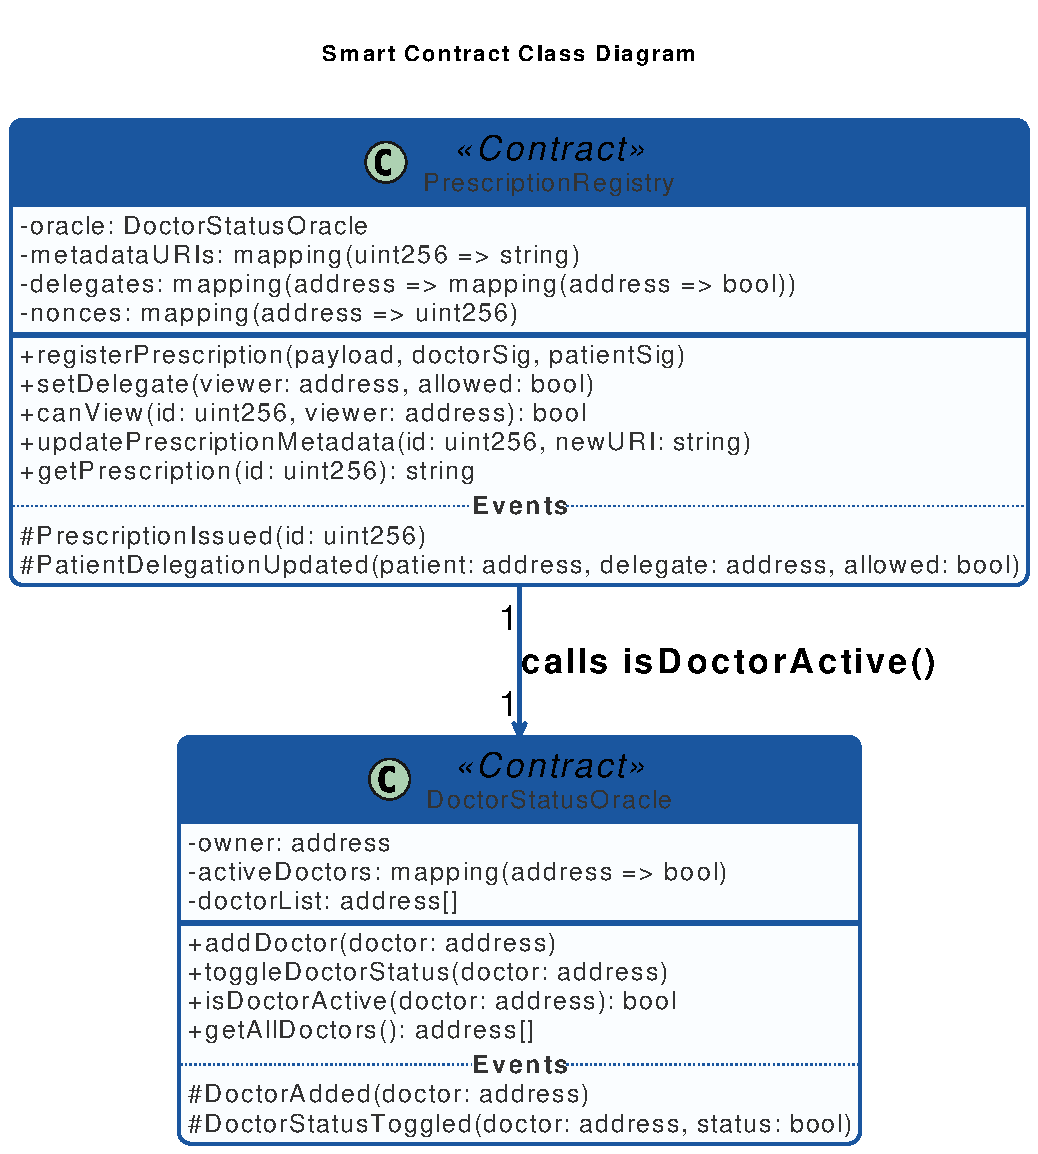
\includegraphics[width=0.95\textwidth]{smart_contract_uml.pdf}
    \caption{UML Class Diagram of the Smart Contract Layer showing state variables, functions, and the oracle dependency.}
    \label{fig:contract_uml}
\end{figure}
\clearpage

\subsection{PrescriptionRegistry.sol}

The \texttt{PrescriptionRegistry} contract is the operational core of the proposed system.
It anchors encrypted prescription metadata on-chain, verifies the dual-signature
publication rule, and enforces patient controlled delegation. In the current
implementation, pending approvals are managed off-chain in the request queue;
only fully approved prescriptions and access control state are committed to the
blockchain. The contract is authored in Solidity 0.8.23, which provides built in
integer overflow protection. State-changing operations emit events that form an
on-chain audit trail accessible to any party.

The contract exposes the following primary functions:

\begin{itemize}
  \item \textbf{\texttt{registerPrescription(...)}} -
    The primary publication entrypoint. It checks the doctor's status in the
    \texttt{DoctorStatusOracle}, enforces a non-zero patient address, validates
    the expiry against \texttt{block.timestamp}, computes the EIP-712 digest,
    recovers both signers using \texttt{ecrecover}, advances the doctor's nonce,
    stores the \texttt{metadataURI}, and emits \texttt{PrescriptionIssued}. No
    plaintext record payload is ever written on-chain.
  \item \textbf{\texttt{setDelegate(address viewer, bool allowed)}} - Patient
    grants or revokes blanket read access for a specified address. Emits
    \texttt{PatientDelegationUpdated}, which is later reflected in the client-side
    access-management workflow.
  \item \textbf{\texttt{canView(uint256 id, address viewer)}} - A pure view
    function encoding all access logic: returns \texttt{true} if the viewer is
    the prescribing doctor, the patient, or an active delegate. Called by the
    backend before returning any CID to an API caller.
  \item \texttt{updatePrescriptionMetadata(uint256 id, string newURI)} - Updates the on-chain CID reference after re-encryption has produced a new IPFS bundle with an additional recipient entry. Crucially, this function enforces a strict \texttt{require(msg.sender == prescriptions[id].patient)} access control check. This guarantees that only the cryptographically verified patient who owns the prescription can authorize an update to its underlying storage pointer, preventing delegates, doctors, or malicious actors from hijacking the record's metadata.
  \item \textbf{\texttt{getPrescription(uint256 id)}} - Returns the stored
    on-chain metadata for an authorised caller and reverts for unauthorised
    viewers, ensuring that CID retrieval remains aligned with contract access rules.
\end{itemize}

\subsection{DoctorStatusOracle.sol}

The \texttt{DoctorStatusOracle} contract was introduced in the final development
cycle to eliminate any reliance on off-chain physician verification. It maintains
a transparent, on-chain registry of physician wallet addresses and their active
status, administered by a designated contract owner.

\begin{itemize}
  \item \textbf{\texttt{addDoctor(address)}} - Owner-only function that registers
    a new physician address and sets their status to active. Emits \texttt{DoctorAdded}.
  \item \textbf{\texttt{toggleDoctorStatus(address)}} - Owner-only function that
    flips the active/suspended status of a registered physician. Emits
    \texttt{DoctorStatusToggled}. This enables real-time credential revocation
    without requiring a contract upgrade or redeployment.
  \item \textbf{\texttt{isDoctorActive(address)}} - Public view function called
    by \texttt{PrescriptionRegi-\\stry} inside \texttt{registerPrescription()}. Returns
    \texttt{false} for any address that has not been registered or has been suspended.
  \item \textbf{\texttt{getAllDoctors()}} - Returns the complete array of registered
    addresses for display in the administrator panel.
\end{itemize}

All administrative actions emit on-chain events, creating a fully auditable history
of every credential management decision. This transparency partially mitigates the
concern that the admin account represents a centralised trust anchor.

\section{End-to-End Encryption}

\begin{frame}{}
\begin{figure}
\centering
% Constrains the taller flowchart to fit perfectly above the text
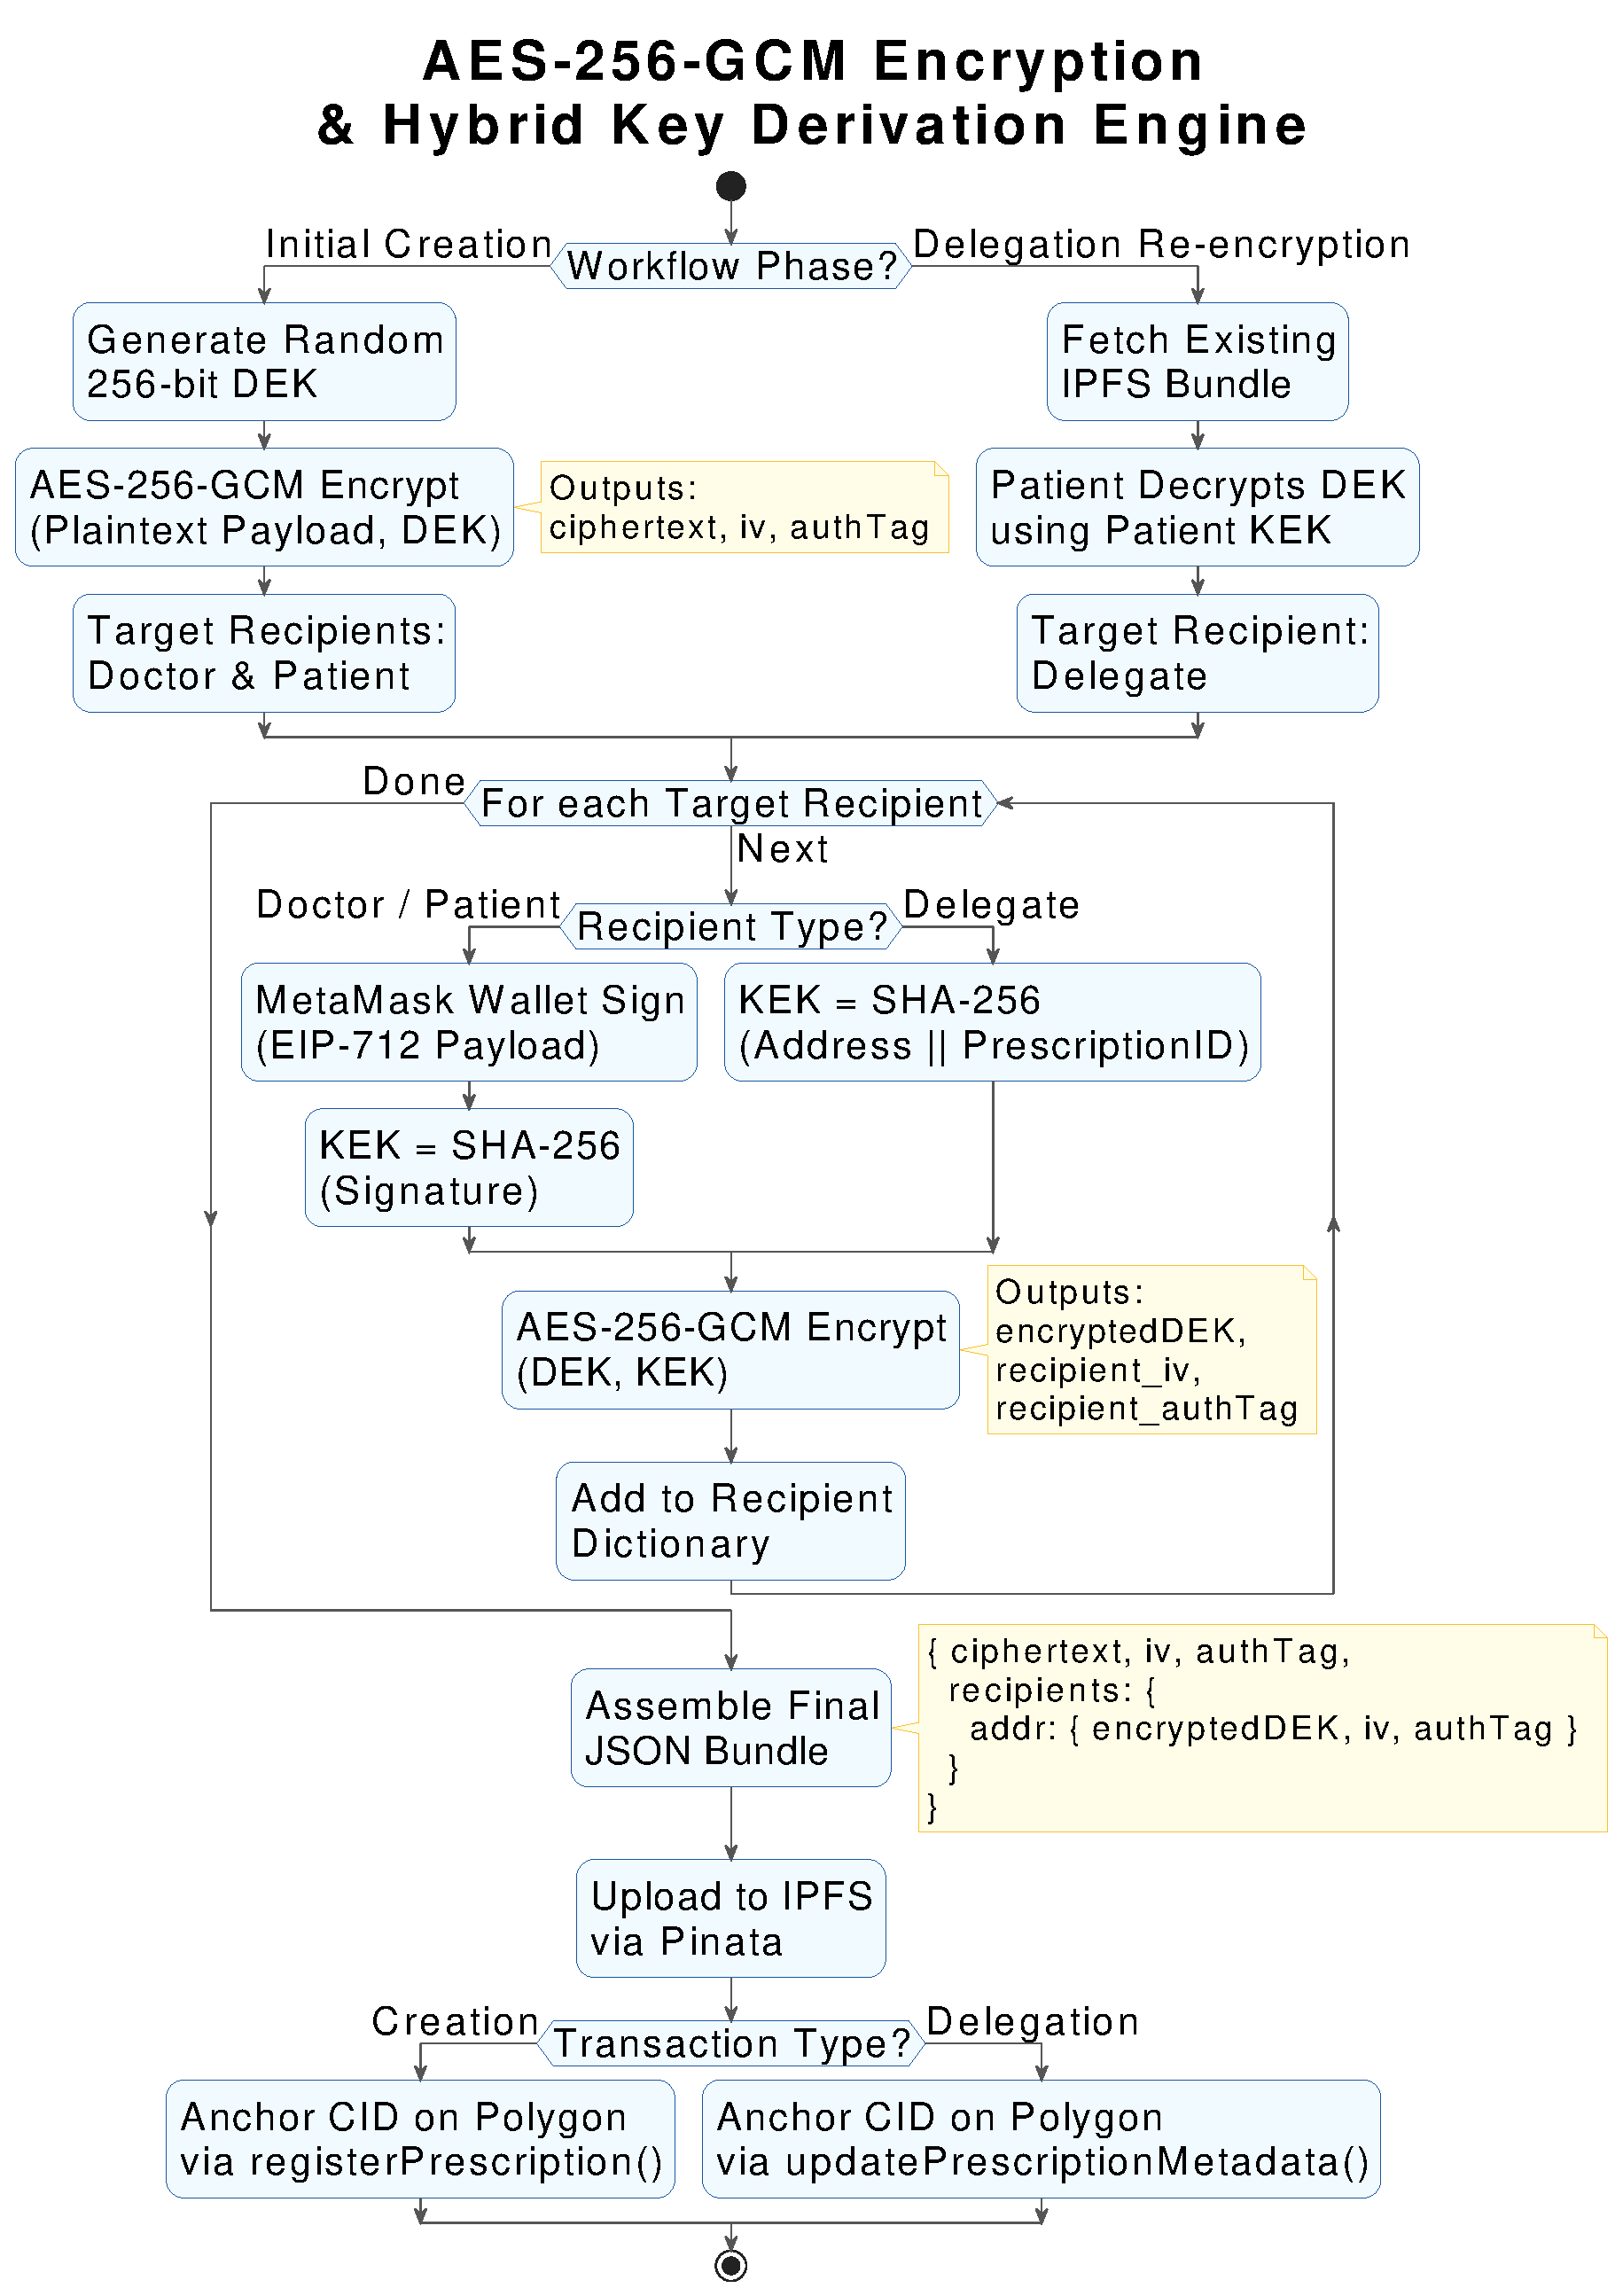
\includegraphics[height=0.68\textheight, keepaspectratio]{endToEnd_encryption.pdf}
\end{figure}

\vspace{0.1cm}
\small
\begin{itemize}
  \item At creation, a single DEK encrypts the payload, and wallet signatures derive KEKs for the Doctor and Patient[cite: 1].
  \item During delegation, the Patient decrypts the DEK client-side and derives a new KEK for the delegate using their public address[cite: 1].
  \item The updated bundle generates a new CID, which is anchored via \texttt{updatePrescriptionMetadata()}[cite: 1].
\end{itemize}
\end{frame}
\subsection{Architecture and Design Rationale}

The end-to-end encryption system was designed around a single non negotiable
requirement: the main prescription workflow should avoid exposing plaintext medical
data beyond the user's browser wherever possible. This is achieved by executing
encryption and decryption logic within the user's web browser using the Web Crypto
API and by storing only encrypted bundles plus CIDs off-chain. Even so, the
current prototype retains compatibility paths that can accept plaintext request
payloads during development, so the design should be described as encrypted first
rather than as a formally strict zero knowledge backend.

The encryption primitive is AES-256-GCM (Advanced Encryption Standard in
Galois/Counter Mode with a 256-bit key). GCM mode provides authenticated
encryption: it simultaneously ensures confidentiality via AES, integrity via the
96-bit GCM authentication tag, and resistance to chosen ciphertext attacks. Any
modification to the ciphertext will cause the authentication tag check to fail
on decryption.

A multi-recipient key architecture allows a single encrypted document to be
independently decrypted by multiple authorised parties:

\begin{itemize}
  \item A fresh random 256-bit \textbf{Data Encryption Key (DEK)} is generated
    for each prescription. The plaintext is encrypted once with this DEK.
  \item For each authorised recipient, a \textbf{Key Encryption Key (KEK)} is
    derived independently and used to encrypt a copy of the DEK. The resulting
    per-recipient \texttt{encryptedDEK} entries are bundled alongside the
    ciphertext in the IPFS JSON blob.
  \item To decrypt, an authorised recipient derives their KEK, decrypts their
    \texttt{encryptedDEK} to recover the shared DEK, and uses the DEK to decrypt
    the ciphertext.
\end{itemize}

\subsection{Hybrid Key Derivation}


\begin{enumerate}
  \item \textbf{EIP-712 Signature-based (Doctor and Patient):}
    \[ \text{KEK} = \text{SHA256}(\sigma_{\text{EIP712}}) \]
    The KEK is derived by hashing an EIP-712 structured-data signature produced
    by the recipient's MetaMask wallet. Security rests on the secrecy of the
    wallet's private key: the KEK is derived on-demand whenever the user signs,
    and is never stored, cached, or transmitted. Two users with different wallets
    will always produce different KEKs for the same prescription.

  \item \textbf{Address-based (Delegates):}
    \[ \text{KEK} = \text{SHA256}(\text{walletAddress} \,\|\, \text{prescriptionId}) \]
    For delegated recipients added after the prescription was created, the KEK
    is derived deterministically from the delegate's public wallet address and
    the prescription identifier. This derivation requires no active session from
    the delegate and can be performed by the component carrying out the delegated
    bundle update; in the current prototype that update is driven from the client
    after patient approval. The delegate derives the same KEK client-side when
    they later access the record.
\end{enumerate}

\subsection{Encryption Flow}

\begin{enumerate}
  \item Physician completes the prescription form. Browser generates a random 256-bit DEK.
  \item Prescription JSON is encrypted with the DEK using AES-256-GCM:\\          
    $\texttt{(ciphertext, iv, authTag)} \leftarrow \text{AES-GCM}_{DEK}(\text{plaintext})$.
  \item For each authorised recipient (doctor, patient), a KEK is derived and the
    DEK is encrypted: $\texttt{encryptedDEK}_r \leftarrow \text{AES-GCM}_{KEK_r}(DEK)$.
  \item All components are assembled into a JSON bundle:
    $\{ \texttt{ciphertext}, \texttt{iv}, \texttt{authTag}, \\
    \texttt{recipients}: \{ addr: \{ \texttt{encryptedDEK}, \texttt{iv}, \texttt{authTag} \} \} \}$.
  \item Bundle is pinned to IPFS via Pinata, yielding a CID.
  \item CID is stored on-chain as \texttt{metadataURI} via \texttt{registerPrescription()}.
\end{enumerate}

\subsection{Decryption Flow}

\begin{enumerate}
  \item Authorised user requests a prescription; backend calls \texttt{canView()} on-chain and returns the CID.
  \item Browser fetches the encrypted bundle directly from IPFS using the CID.
  \item User derives their KEK client-side (EIP-712 signature or address based).
  \item Browser decrypts \texttt{encryptedDEK} with KEK to recover the plaintext DEK.
  \item Browser decrypts ciphertext with DEK; GCM authentication tag is verified as part of this step, rejecting any tampered ciphertext.
\end{enumerate}

\subsection{Core Integrity Formulae}

The blockchain and storage integrity claims in the proposed system rely on a small set of
hash-based relationships that are simple enough to state explicitly:

\begin{align*}
\mathtt{dataHash} &= H(\mathtt{encryptedBundle}) \\
\mathtt{cid} &\approx H(\mathtt{encryptedBundle}) \\
\mathtt{blockHash} &= H(\mathtt{index} \| \mathtt{timestamp} \| \mathtt{previousHash} \| \mathtt{dataHash} \| \mathtt{metadataURI})
\end{align*}

In words, any modification to the encrypted record changes the content hash,
which changes the CID, which in turn breaks the consistency of the on-chain
anchor if the old CID is still referenced. If a historical block is modified,
its \texttt{blockHash} changes, and the next block's stored \texttt{previousHash}
no longer matches. This is the core reason blockchain history is tamper-evident.

\section{EIP-712 Dual-Signature Workflow}

EIP-712 is an Ethereum standard for hashing and signing typed structured data.
Prior to EIP-712, most wallet signing operations presented users with an opaque
hexadecimal hash, providing no human readable context about what was being signed
and creating a significant phishing attack surface. EIP-712 resolves this by
structuring the signed payload into labelled fields that MetaMask displays in
plain language before the user confirms. In the context of the proposed system, this means the
patient sees the full prescription content physician name, medication, dosage,
and duration before co-signing, constituting genuine informed consent at the
cryptographic protocol level.

The dual-signature flow proceeds as follows:

\begin{enumerate}
  \item Physician fills the prescription form and signs the EIP-712 payload
    (\texttt{doctor}, \texttt{patient}, \texttt{medicationDetails}, \texttt{nonce},
    \texttt{validUntil}) via MetaMask, producing \texttt{doctorSig}. The prescription
    is simultaneously encrypted client side and uploaded to IPFS.
  \item The backend stores a pending request containing the encrypted bundle
    reference, doctor signature material, and patient address so the patient can
    review it later.
  \item Patient opens the pending request in their dashboard. The browser fetches
    and decrypts the bundle client side. The patient reviews the plaintext
    prescription in their browser.
  \item If approved, the patient signs the same EIP-712 payload via MetaMask,
    producing \texttt{patientSig}, and submits \texttt{registerPrescription()} on-chain.
  \item The contract recovers the signer addresses from both signatures using
    \texttt{ecrecover}, verifies they match the expected doctor and patient
    addresses, checks the nonce has not been used, validates the expiry, and
    confirms the doctor's oracle status. If all checks pass, the prescription is
    permanently committed; otherwise the transaction reverts.
\end{enumerate}

Security properties: per-prescription nonces prevent signature replay; expiry
timestamps limit the window for delayed submission attacks; domain separation
prevents cross-contract or cross application signature reuse; and on-chain ECDSA
verification requires no private key disclosure.

\section{Automatic Re-encryption}

When a patient calls \texttt{setDelegate(addr, true)}, the system must ensure
that the new delegate can decrypt all of the patient's existing prescription
records - records that were encrypted before the delegate existed. In the current
prototype this is achieved through a client-driven update workflow:

\begin{enumerate}
  \item Patient grants the delegate on-chain using \texttt{setDelegate(addr, true)}.
  \item The frontend queries all prescriptions visible to the patient and filters
    those whose metadata points to encrypted bundles.
  \item For each prescription, the browser fetches the encrypted bundle from IPFS,
    decrypts the DEK using the patient's KEK, computes the delegate's derived KEK,
    encrypts the DEK for the delegate, appends the new recipient entry to the bundle,
    and uploads the updated bundle to IPFS.
  \item The patient then submits \texttt{updatePrescriptionMetadata()} on-chain
    with the new CID for each updated prescription.
\end{enumerate}

The current implementation processes these records iteratively with explicit client side progress tracking and per-record error capture. Because each historical record update strictly requires an IPFS fetch, a client side KEK derivation, a Pinata IPFS repin (averaging 1.28 seconds), and an on-chain \texttt{updatePrescriptionMetadata()} transaction (averaging 1.02 seconds on the local testnet), the baseline overhead is approximately 2.5 seconds per record. Consequently, delegating access to a moderate historical archive of 20 existing prescriptions requires roughly 50 seconds of linear processing time. While the frontend's explicit progress tracking mitigates the immediate user experience impact by preventing silent timeouts, this $O(N)$ iterative bottleneck represents a practical usability constraint for patients with extensive medical histories. A priority future optimisation will decouple this loop by parallelising the off-chain IPFS repinning operations and aggregating the on-chain pointer updates into a single batched smart contract transaction. When the delegate later accesses a prescription, they derive the same address-based KEK clien -side and decrypt normally.

\section{Backend API and Deployment}

\subsection{Core API Endpoints}

\begin{table}[H]
\centering
\caption{Core backend REST endpoints}
\label{tab:api}
\begin{adjustbox}{max width=\textwidth}
\begin{tabular}{@{}p{5.8cm}p{7.2cm}@{}}
\toprule
\textbf{Endpoint} & \textbf{Responsibility} \\
\midrule
\texttt{POST /api/requests} & Create a pending prescription or access request; validate sender and signature metadata; persist the request queue entry and associated encrypted payload reference. \\[4pt]
\texttt{GET /api/requests} & Return all pending and completed requests for the authenticated wallet address. \\[4pt]
\texttt{POST /api/requests/:id/approve} & Record patient approval metadata after the wallet submits the corresponding on-chain transaction. \\[4pt]
\texttt{GET /api/prescriptions/:id} & Verify \texttt{canView()} on-chain and return anchored prescription metadata only to authorised callers. \\[4pt]
\texttt{GET /api/patients/:addr/prescriptions} & List recorded prescriptions visible to the requesting wallet, including on-chain IDs and current \texttt{metadataURI} values. \\[4pt]
\texttt{GET/POST /api/doctors}, \texttt{PUT /api/doctors/:addr/toggle} & Surface oracle managed physician status for the admin flow. \\
\bottomrule
\end{tabular}
\end{adjustbox}
\end{table}

\subsection{Quick Start}

\begin{lstlisting}[language=bash, caption=Full local setup (mirrors the project README)]
git clone https://github.com/U-Shashank/btp && cd btp

# Contracts: install, test, deploy
cd contracts && forge install && forge test
anvil   # start local node in a separate terminal

forge create src/PrescriptionRegistry.sol:PrescriptionRegistry \
  --rpc-url http://127.0.0.1:8545 --private-key <DEPLOYER_KEY>
forge create src/DoctorStatusOracle.sol:DoctorStatusOracle \
  --rpc-url http://127.0.0.1:8545 --private-key <DEPLOYER_KEY>

# Backend
cd ../server && npm install
cp .env.example .env   # set RPC_URL, contract addresses, PINATA_JWT
npm run dev

# Frontend
cd ../web && npm install
cp .env.example .env   # set VITE_* values to match backend
npm run dev            # http://localhost:5173
\end{lstlisting}

\subsection{End-to-End Test Scenario}



\begin{enumerate}
  \item Admin navigates to the Admin Panel and whitelists a physician wallet via the
    \texttt{DoctorStatusOracle} interface.
  \item Doctor logs in, fills the prescription form, and signs the EIP-712 payload;
    the browser encrypts the bundle and the backend records the pending request.
  \item Patient opens the pending request in the dashboard; the browser decrypts
    the bundle client side and displays the plaintext prescription for review.
  \item Patient co-signs the EIP-712 payload via MetaMask and submits
    \texttt{registerPrescription()}; the contract validates both signatures,
    checks expiry and nonce progression, and emits \texttt{PrescriptionIssued}.
  \item The backend stores the resulting transaction hash and \texttt{prescriptionId}
    for later retrieval.
  \item Patient optionally grants access to a delegate; the frontend then
    re-encrypts existing encrypted bundles for the new recipient and updates the
    on-chain \texttt{metadataURI} values.
\end{enumerate}


Figure \ref{fig:happy_path_sequence} visually summarizes this complete dynamic happy path flow, illustrating the sequence of cryptographic handoffs between the actors, the off-chain storage layer, and the Polygon smart contracts.

\begin{figure}[htbp]
    \centering
    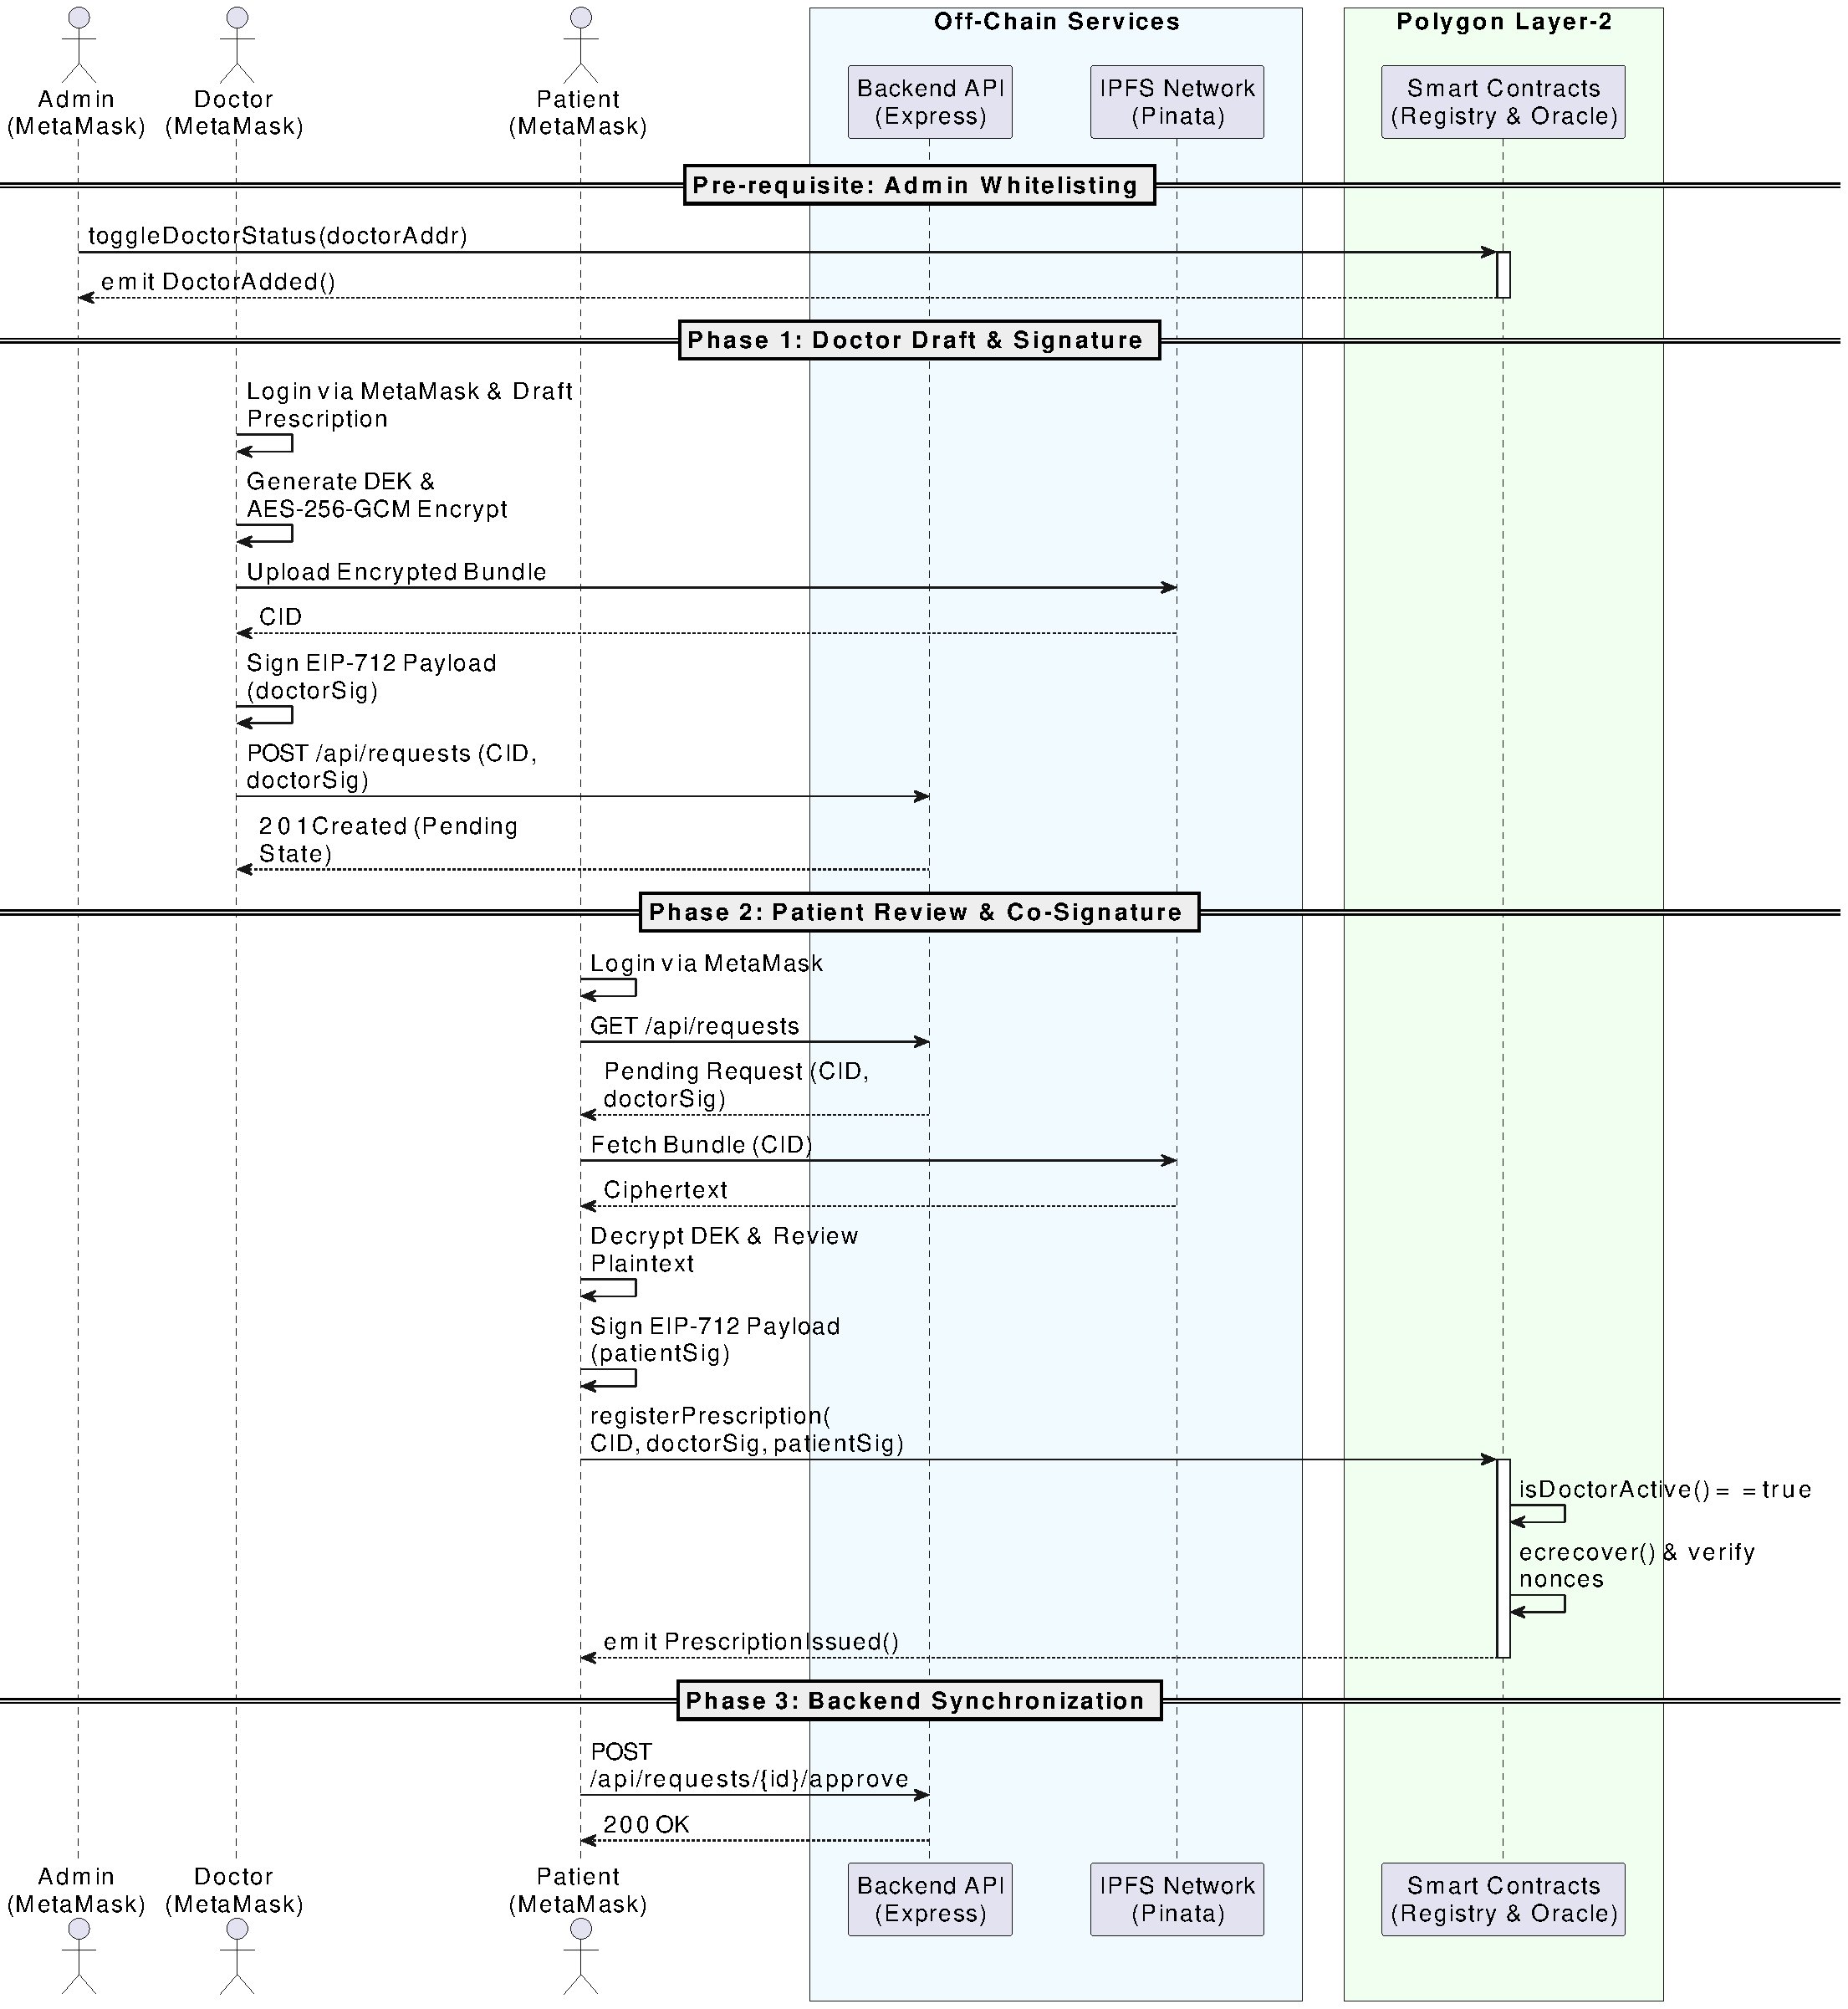
\includegraphics[width=0.98\textwidth]{end_to_end_happy_path.pdf}
    \caption{UML Sequence Diagram illustrating the complete end-to-end happy path, from admin whitelisting to final on-chain commitment.}
    \label{fig:happy_path_sequence}
\end{figure}

% ══════════════════════════════════════════════════════════════════════════════
\chapter{Evaluation}
% ══════════════════════════════════════════════════════════════════════════════

\section{Overview}

The evaluation of the proposed system rests on five pillars: contract correctness and gas
testing, prototype measured performance metrics collected from the running system,
local chain blockchain benchmarking on Anvil, a synthetic dataset used for
integration testing, and simulation based analyses (tamper simulation and workload
projection). Together these provide a comprehensive and honest evidence base that
does not overclaim comparability with multi-node permissioned benchmarks from
the literature.

\section{Experimental Tooling}

\subsection{Synthetic Dataset Generator (\texttt{generate-synthetic-data.js})}

To provide realistic, repeatable integration test data, a deterministic synthetic
dataset generator was built using a seeded linear congruential random number
generator (seed \texttt{20260401}). The deterministic seed ensures that any
reviewer can regenerate an identical dataset and reproduce all downstream
simulation results.

The generator produces a population of 30 patients with realistic Indian names,
ages distributed uniformly between 18 and 78, blood group assignments, and allergy
profiles drawn from six categories (none, penicillin, peanuts, dust, seafood,
pollen). Eight doctors are generated with specialties drawn from eight clinical
disciplines (general medicine, cardiology, dermatology, paediatrics, orthopaedics,
neurology, ENT, pulmonology) and hospital affiliations across five institutions.
Approximately 10\% of doctors are assigned a suspended status, specifically to
exercise the oracle's credential verification logic.

From this population, 120 prescriptions are generated. Each prescription draws a
patient and an active doctor at random, selects a diagnosis from ten categories,
and assigns one to three medications with dosage and schedule information. Workflow
state flags are assigned to reflect realistic distribution: 109 of 120 prescriptions
are patient approved (leaving 11 in a pending state to simulate the patient review
queue), and 24 carry a delegate addition. Each prescription includes a simulated
IPFS CID and an on-chain anchor hash. The dataset is exported to both
\texttt{synthetic-dataset.json} (for programmatic use by the downstream simulation
tools) and \texttt{synthetic-prescriptions.csv} (for tabular inspection).

\subsection{Blockchain Tamper Simulation (\texttt{simulate-blockchain.js})}

To provide empirical grounding for the immutability claim, a blockchain tamper
simulation was developed that constructs a local chain from prescription payloads
and evaluates three adversarial scenarios. Each block's hash is computed as:
\[ \texttt{blockHash} = \text{SHA256}(\texttt{index} \| \texttt{timestamp} \|
\texttt{previousHash} \| \texttt{dataHash} \| \texttt{ipfsCid}) \]
where \texttt{dataHash} is the SHA-256 of the serialised payload. This structure
means that any modification to a payload changes \texttt{dataHash}, which changes
\texttt{blockHash}, which breaks the \texttt{previousHash} link of the successor
block propagating a validation failure through all downstream blocks.

\begin{table}[H]
\centering
\caption{Blockchain tamper simulation results (5-block chain, tamper at block 2)}
\label{tab:tamper}
\begin{tabular}{@{}lcc@{}}
\toprule
\textbf{Scenario} & \textbf{Chain Valid?} & \textbf{Failing Blocks} \\
\midrule
Original chain (no tampering) & \checkmark Yes & 0 \\
Tampered data only (diagnosis rewritten at block 2) & \texttimes No & Blocks 2--5 \\
Tampered + single block rehash (only block 2 rehashed) & \texttimes No & Blocks 3--5 \\
\bottomrule
\end{tabular}
\end{table}

The results confirm that rewriting data in block 2 immediately invalidates that
block and all four successors. An adversary who additionally rehashes only the
tampered block still fails: block 3's \texttt{previousHash} field now contains
a stale value referencing the original block 2 hash. Repairing the cascade would
require recomputing the hash of every successor block and in a live distributed
network, overwriting these blocks would require controlling a majority of the
network's stake, which is computationally infeasible under normal operating conditions.

\subsection{Workload Projection (\texttt{simulate-workload.js})}

The workload simulation script projects cumulative operation costs for three
representative deployment scenarios by multiplying prototype measured per-operation
averages against workload sizes. Averages are read from \texttt{prototype-baseline.json}
(populated by the live metrics logging in \texttt{server/metrics/data.json}) and
the average payload size from the synthetic dataset.

The underlying cumulative estimates follow the simple relationships:

\begin{align*}
\mathtt{cumulativeDraftTime} &\approx \mathtt{prescriptionCount} \times \overline{\mathtt{draftCreationTime}} \\
\mathtt{cumulativeFinalizeTime} &\approx \mathtt{prescriptionCount} \times \overline{\mathtt{finalizationTime}} \\
\mathtt{estimatedTotalGas} &\approx (\mathtt{prescriptionCount} \times \overline{\mathtt{registerGas}}) \\
\qquad {}+ (\mathtt{delegateCount} \times \overline{\mathtt{delegateGas}})
\end{align*}

These expressions do not model network contention or validator consensus delay;
they are workload projections grounded in the current prototype averages.

\begin{table}[H]
\centering
\caption{Workload projection based on prototype-measured averages}
\label{tab:workload}
\begin{adjustbox}{max width=\textwidth}
\begin{tabular}{@{}lp{2.0cm}p{2.2cm}p{2.2cm}p{2.4cm}@{}}
\toprule
\textbf{Workload} & \textbf{Prescrip-tions} & \textbf{Cumul.\ Draft (s)} & \textbf{Cumul.\ Finalize (s)} & \textbf{Off-chain Volume (MB)} \\
\midrule
Pilot review demo         & 25  & 334.5  & 319.75   & $\sim$0.007 \\
Department rollout        & 100 & 1338.0 & 1279.0   & $\sim$0.026 \\
Hospital scale simulation & 500 & 6690.0 & 6395.0  & $\sim$0.131 \\
\bottomrule
\end{tabular}
\end{adjustbox}
\end{table}

The projections confirm approximately linear cumulative growth: increasing the
number of prescriptions increases the total measured draft, finalisation, and gas
costs proportionally. Under the current local baseline, hospital scale simulation
(500 prescriptions) yields large sequential cumulative times because the prototype
measurements already include user driven signing, encryption, API, and IPFS
overhead. These values should therefore be interpreted as workload projections
grounded in prototype averages, not as throughput benchmarks. The off-chain volume
remains small because only compact encrypted JSON bundles are being modelled.

\begin{figure}[p]
\centering
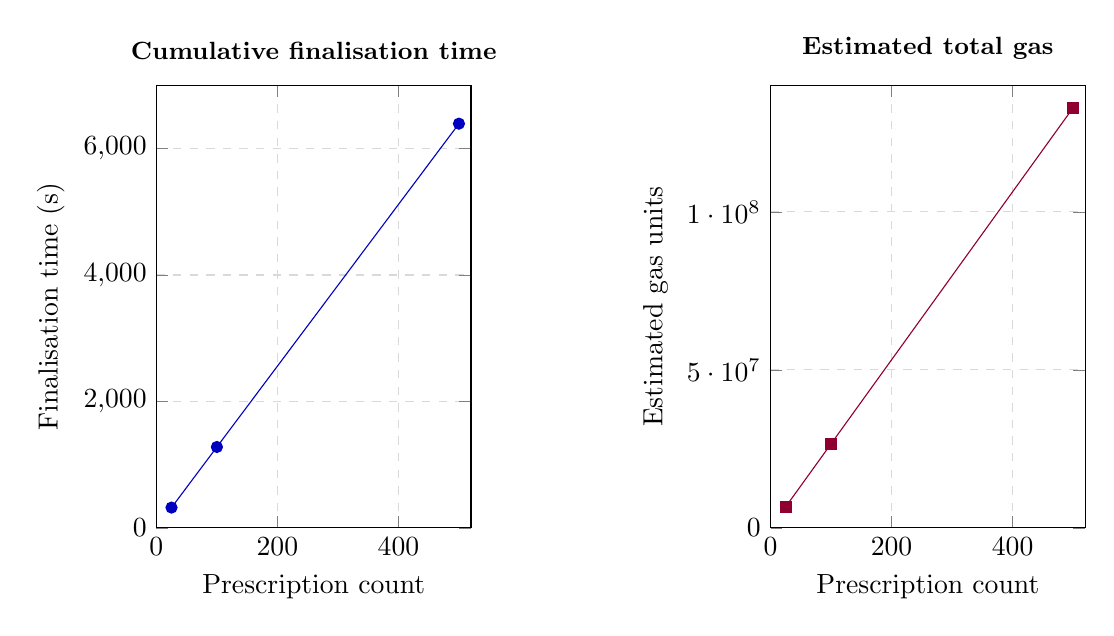
\begin{tikzpicture}
\begin{axis}[
  width=0.46\textwidth,
  height=7.2cm,
  xlabel={Prescription count},
  ylabel={Finalisation time (s)},
  xmin=0,
  xmax=520,
  ymin=0,
  ymax=7000,
  grid=major,
  grid style={dashed, gray!30},
  title={Cumulative finalisation time},
  title style={font=\small\bfseries},
  at={(0cm,0cm)},
]
\addplot[color=blue!75!black, mark=*] coordinates {
  (25,319.75) (100,1279.0) (500,6395.0)
};
\end{axis}
\begin{axis}[
  width=0.46\textwidth,
  height=7.2cm,
  xlabel={Prescription count},
  ylabel={Estimated gas units},
  xmin=0,
  xmax=520,
  ymin=0,
  ymax=140000000,
  scaled y ticks=false,
  grid=major,
  grid style={dashed, gray!30},
  title={Estimated total gas},
  title style={font=\small\bfseries},
  at={(7.8cm,0cm)},
]
\addplot[color=purple!75!black, mark=square*] coordinates {
  (25,6646080) (100,26584320) (500,132921600)
};
\end{axis}
\end{tikzpicture}
\caption{Workload simulation scaling trends derived from prototype-measured averages}
\label{fig:workload-plots}
\end{figure}

\subsection{Local-Chain Load Benchmark (\texttt{anvil-load-test.js})}

To isolate blockchain layer behaviour from frontend, encryption, and IPFS overhead,
a dedicated Anvil benchmark script repeatedly submits real \texttt{registerPrescription()}
and \texttt{setDelegate()} transactions against a fresh local deployment. The
benchmark supports both quiet sequential traffic and burst traffic with delayed
block production, allowing the report to separate ``cost per transaction on a
quiet chain'' from ``confirmation latency under contention''.

Throughput in this benchmark is reported as:

\[
\mathtt{throughput} = \frac{\mathtt{successfulTransactions}}{\mathtt{totalWallClockTime}}
\]

\begin{table}[H]
\centering
\caption{Representative local-chain benchmark results from the verification run}
\label{tab:anvil-load}
\begin{adjustbox}{max width=\textwidth}
\begin{tabular}{@{}lcccc@{}}
\toprule
\textbf{Operation / Mode} & \textbf{Tx count} & \textbf{Avg.\ Latency (ms)} & \textbf{Avg.\ Gas} & \textbf{Throughput (tx/s)} \\
\midrule
\texttt{registerPrescription} / sequential & 5 & 969.8 & 148552.8 & 1.02 \\
\texttt{registerPrescription} / burst      & 5 & 1148.2 & 148543.2 & 2.14 \\
\texttt{setDelegate} / sequential          & 5 & 963.2 & 46340.0 & 1.03 \\
\texttt{setDelegate} / burst               & 5 & 1135.6 & 46340.0 & 2.19 \\
\bottomrule
\end{tabular}
\end{adjustbox}
\end{table}


The seemingly counterintuitive observation in Table 5.3---where burst mode yields a higher average individual latency (1148.2 ms vs 969.8 ms) but simultaneously doubles the throughput (2.14 tx/s vs 1.02 tx/s)---is a direct result of how transactions are dispatched to the mempool and how the total wall-clock time denominator is measured. In sequential mode, the benchmark script waits for the cryptographic confirmation of transaction $N$ before dispatching $N+1$. This means the total wall-clock time includes the network round trip and block-mining delay for every individual transaction in sequence. In burst mode, all transactions are injected into the local node's mempool simultaneously. While individual transactions experience higher latency as they sit in the queue waiting for block inclusion (causing the average latency to rise), the EVM is able to pack multiple pending transactions into a single block. Consequently, the total wall-clock time required to clear the entire batch is significantly shorter than waiting for sequential round trips. This shrinks the denominator in the throughput calculation, resulting in a higher transactions-per-second (tx/s) yield and confirming that the system successfully benefits from standard blockchain batching under load.

These results come from a single node local chain and should be interpreted
accordingly. They are useful because they isolate blockchain confirmation cost
from browser signing prompts, encryption, and Pinata uploads, but they do not
constitute a multi node validator benchmark. The burst mode is the more relevant
stress configuration because it begins to expose queueing once transactions are
offered faster than blocks are mined.

\begin{figure}[p]
\centering
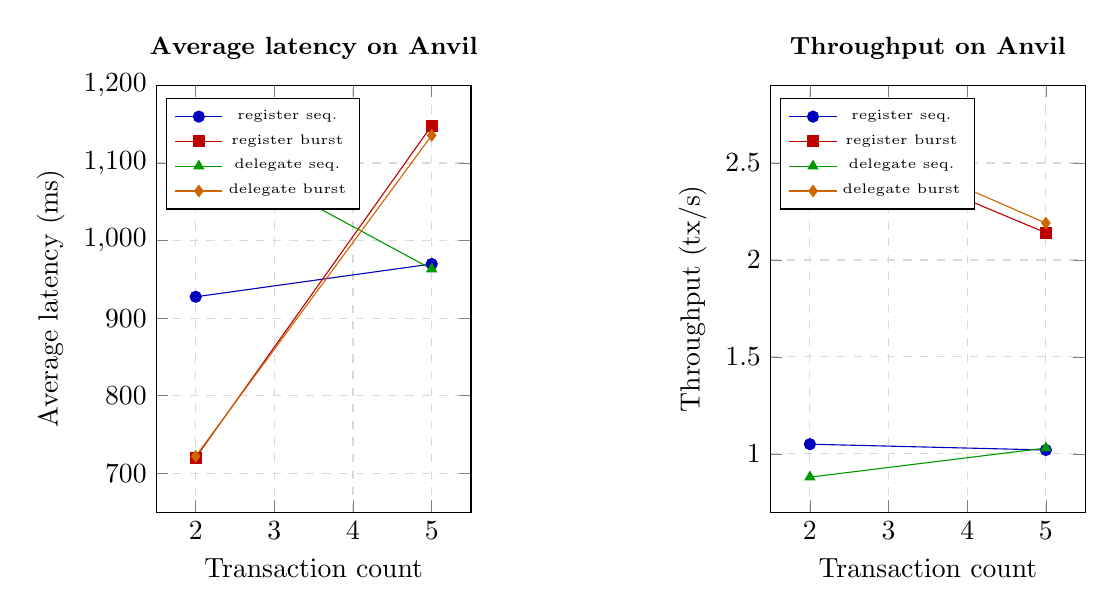
\begin{tikzpicture}
\begin{axis}[
  width=0.46\textwidth,
  height=7.0cm,
  xlabel={Transaction count},
  ylabel={Average latency (ms)},
  xmin=1.5, xmax=5.5,
  ymin=650, ymax=1200,
  grid=major,
  grid style={dashed, gray!30},
  title={Average latency on Anvil},
  title style={font=\small\bfseries},
  legend style={font=\tiny},
  legend pos=north west,
  at={(0cm,0cm)},
]
\addplot[color=blue!75!black, mark=*] coordinates {(2,927.5) (5,969.8)};
\addlegendentry{register seq.}
\addplot[color=red!75!black, mark=square*] coordinates {(2,720.0) (5,1148.2)};
\addlegendentry{register burst}
\addplot[color=green!60!black, mark=triangle*] coordinates {(2,1127.5) (5,963.2)};
\addlegendentry{delegate seq.}
\addplot[color=orange!80!black, mark=diamond*] coordinates {(2,722.0) (5,1135.6)};
\addlegendentry{delegate burst}
\end{axis}
\begin{axis}[
  width=0.46\textwidth,
  height=7.0cm,
  xlabel={Transaction count},
  ylabel={Throughput (tx/s)},
  xmin=1.5, xmax=5.5,
  ymin=0.7, ymax=2.9,
  grid=major,
  grid style={dashed, gray!30},
  title={Throughput on Anvil},
  title style={font=\small\bfseries},
  legend style={font=\tiny},
  legend pos=north west,
  at={(7.8cm,0cm)},
]
\addplot[color=blue!75!black, mark=*] coordinates {(2,1.05) (5,1.02)};
\addlegendentry{register seq.}
\addplot[color=red!75!black, mark=square*] coordinates {(2,2.65) (5,2.14)};
\addlegendentry{register burst}
\addplot[color=green!60!black, mark=triangle*] coordinates {(2,0.88) (5,1.03)};
\addlegendentry{delegate seq.}
\addplot[color=orange!80!black, mark=diamond*] coordinates {(2,2.72) (5,2.19)};
\addlegendentry{delegate burst}
\end{axis}
\end{tikzpicture}
\caption{Latency and throughput from the local-chain Anvil benchmark}
\label{fig:anvil-plots}
\end{figure}

\section{Security Layer Visualisation}

Figure~\ref{fig:security} depicts the five independent security layers and the
threats they address.

% ── FIGURE 5: Security Layers Diagram ────────────────────────────────────────
\begin{figure}[H]
\centering
\begin{tikzpicture}

% Draw concentric rounded rectangles (inside-out)
% Layer 5 – Application (outermost)
\node[secring=darkgray, minimum width=13.0cm, minimum height=7.6cm] (L5) at (0,0) {};
\node[font=\tiny\bfseries, text=darkgray!80] at (0, 3.58)
  {LAYER 5 --- APPLICATION: HTTPS · Zod validation · Client-side encryption only};

% Layer 4 – Storage
\node[secring=accentgreen, minimum width=11.2cm, minimum height=6.3cm] (L4) at (0,-0.2) {};
\node[font=\tiny\bfseries, text=accentgreen!80] at (0, 2.75)
  {LAYER 4 --- STORAGE: IPFS content addressing · GCM auth-tag · Pinata availability};

% Layer 3 – Cryptography
\node[secring=primaryblue, minimum width=9.4cm, minimum height=5.0cm] (L3) at (0,-0.4) {};
\node[font=\tiny\bfseries, text=primaryblue!80] at (0, 1.92)
  {LAYER 3 --- CRYPTOGRAPHY: AES-256-GCM · SHA-256 KEK · ECDSA signatures};

% Layer 2 – Smart Contracts
\node[secring=accentorange, minimum width=7.6cm, minimum height=3.7cm] (L2) at (0,-0.6) {};
\node[font=\tiny\bfseries, text=accentorange!80] at (0, 1.09)
  {LAYER 2 --- SMART CONTRACTS: RBAC · Oracle verify · Nonce replay protect};

% Layer 1 – Blockchain (innermost)
\node[secring=primaryblue, fill=lightblue!40,
      minimum width=5.8cm, minimum height=2.4cm] (L1) at (0,-0.8) {};
\node[font=\small\bfseries, text=primaryblue!90, align=center] at (0,-0.8)
  {LAYER 1 --- BLOCKCHAIN\\Polygon PoS · Immutability · Audit trail};

% ── Threat labels outside ────────────────────────────────────────────────────
\node[font=\tiny, text=darkgray!70, align=center] at (0, -4.6)
  {\textit{Threats addressed outward: Phishing, MITM, Input injection, Tampered IPFS bundles,}\\
   \textit{Key compromise, Smart contract bugs, Doctor impersonation, Replay attacks}};

\end{tikzpicture}
\caption{Five-layer defence-in-depth security architecture of the proposed system}
\label{fig:security}
\end{figure}


\section{Feature Progression}

\begin{table}[H]
\centering
\caption{Feature delivery across review cycles}
\label{tab:progress}
\begin{tabular}{@{}lcc@{}}
\toprule
\textbf{Feature} & \textbf{Review 3} & \textbf{Review 4 (Final)} \\
\midrule
Dual-signature workflow               & \checkmark & \checkmark \\
IPFS off-chain storage                & \checkmark & \checkmark \\
Patient delegation                    & \checkmark & \checkmark \\
React + MetaMask frontend             & \checkmark & \checkmark \\
Local Anvil testnet deployment        & \checkmark & \checkmark \\
End-to-end AES-256-GCM encryption     & \texttimes & \checkmark \\
DoctorStatusOracle contract           & \texttimes & \checkmark \\
Hybrid KEK derivation                 & \texttimes & \checkmark \\
Automatic re-encryption               & \texttimes & \checkmark \\
On-chain EIP-712 dual-signature       & \texttimes & \checkmark \\
Nonce-based replay protection         & \texttimes & \checkmark \\
Admin panel for doctor management     & \texttimes & \checkmark \\
\bottomrule
\end{tabular}
\end{table}

The transition from Review 2 to Review 3 represents a qualitative shift from a
feature-complete functional prototype to a security-hardened research prototype.
Every major security vulnerability identified at Review 2 the absence of
client-side encryption, the lack of physician credential verification, and the
risk of replay attacks was fully resolved in the final iteration, while all
existing functionality was preserved.

\section{Performance Metrics}

All measurements were collected on the Anvil local testnet running on a standard
development workstation. Pinata latencies represent averages over multiple calls
and are subject to internet connectivity variability.

\begin{table}[H]
\centering
\caption{Prototype-measured performance metrics (Anvil local testnet)}
\label{tab:perf}
\begin{adjustbox}{max width=\textwidth}
\begin{tabular}{@{}ll@{}}
\toprule
\textbf{Metric} & \textbf{Observed Value} \\
\midrule
Draft creation workflow                  & 13.38~s \\
Finalisation workflow                    & 12.79~s \\
Delegate approval workflow               & 7.99~s \\
Pinata IPFS upload latency               & 1.28~s \\
Encryption time                          & 4.90~s \\
Decryption time                          & 14~ms \\
API latency overall                      & 19.95~ms mean, 5.30~ms median, 37.41~ms p95 \\
Integrated \texttt{registerPrescription} gas & 256{,}532 gas \\
Integrated \texttt{setDelegate} gas      & 46{,}556 gas \\
Forge smart-contract test suite          & 37 / 37 tests passed \\
\bottomrule
\end{tabular}
\end{adjustbox}
\end{table}

These values are prototype observations collected under local conditions rather
than large sample distributed benchmarks. The main takeaway is that full workflow
latency is dominated by off-chain work such as wallet interaction, browser-side
encryption, and IPFS upload, whereas the blockchain only benchmark isolates a
smaller contract confirmation component. The low API median indicates that the
Express layer itself is not the main bottleneck in the current prototype.

\begin{figure}[p]
\centering
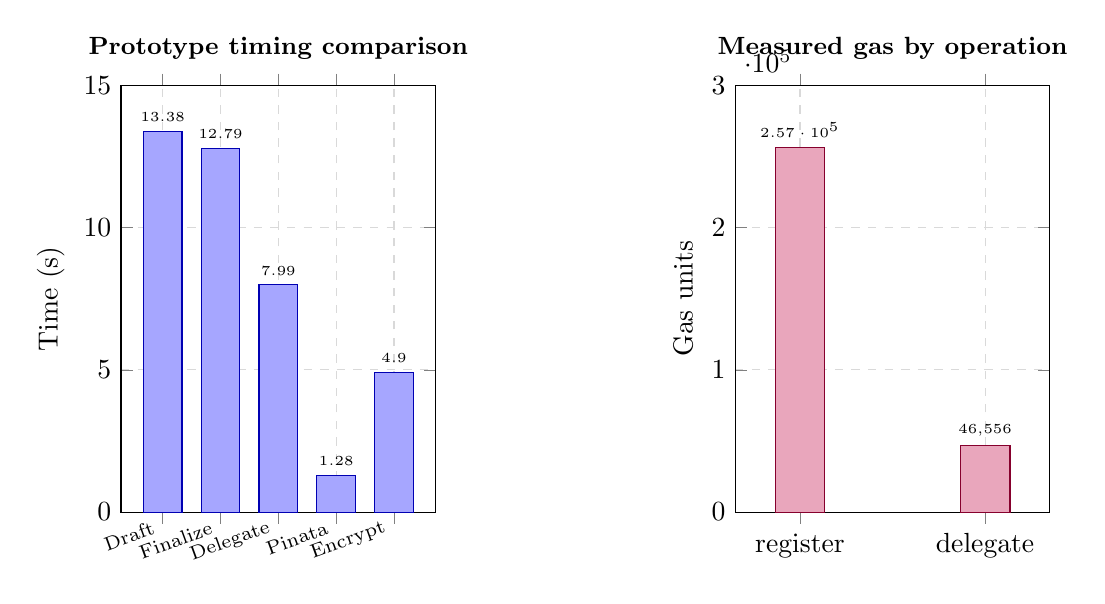
\begin{tikzpicture}
\begin{axis}[
  ybar,
  width=0.46\textwidth,
  height=7.0cm,
  ymin=0,
  ymax=15,
  ylabel={Time (s)},
  symbolic x coords={Draft,Finalize,Delegate,Pinata,Encrypt},
  xtick=data,
  xticklabel style={font=\scriptsize, rotate=20, anchor=east},
  nodes near coords,
  nodes near coords style={font=\tiny},
  bar width=14pt,
  enlarge x limits=0.18,
  grid=major,
  grid style={dashed, gray!30},
  title={Prototype timing comparison},
  title style={font=\small\bfseries},
  at={(0cm,0cm)},
]
\addplot[fill=blue!35, draw=blue!70!black] coordinates {
  (Draft,13.38) (Finalize,12.79) (Delegate,7.99) (Pinata,1.28) (Encrypt,4.90)
};
\end{axis}
\begin{axis}[
  ybar,
  width=0.46\textwidth,
  height=7.0cm,
  ymin=0,
  ymax=300000,
  ylabel={Gas units},
  symbolic x coords={register,delegate},
  xtick=data,
  nodes near coords,
  nodes near coords style={font=\tiny},
  bar width=18pt,
  enlarge x limits=0.35,
  grid=major,
  grid style={dashed, gray!30},
  title={Measured gas by operation},
  title style={font=\small\bfseries},
  at={(7.8cm,0cm)},
]
\addplot[fill=purple!35, draw=purple!70!black] coordinates {
  (register,256532) (delegate,46556)
};
\end{axis}
\end{tikzpicture}
\caption{Prototype timing and measured gas for the proposed system}
\label{fig:prototype-plots}
\end{figure}



\section{Security Evaluation}

Security evaluation was conducted through a combination of automated Forge tests
and manual adversarial testing against the running prototype:

\begin{itemize}
  \item \textbf{Unauthorised Access:} Requests from wallets not authorised for
    a given prescription were sent directly to \texttt{GET /api/prescriptions/:id}.
    In every case, the backend's \texttt{canView()} check returned \texttt{false}
    and the response was \texttt{HTTP 403 Forbidden}. No CID, metadata, or
    prescription content was disclosed to any unauthorised caller.
  \item \textbf{Role Enforcement:} Forge tests confirmed that
    \texttt{registerPrescription()} rejects inactive or unknown doctors, invalid
    signatures, and expired payloads, while \texttt{updatePrescriptionMetadata()}
    rejects callers other than the designated patient.
  \item \textbf{Replay Attack:} A complete set of EIP-712 signatures captured from
    a successful \texttt{registerPrescription()} transaction was replayed in a new
    transaction. The contract's nonce progression caused the replayed signatures
    to no longer match the newly computed digest, and the call reverted during
    signature verification.
  \item \textbf{IPFS Integrity:} An encrypted bundle was manually modified on IPFS
    and the original CID was used to access it. The modified CID did not match the
    on-chain reference. Additionally, the AES-GCM authentication tag verification
    during client side decryption rejected the tampered ciphertext, confirming
    dual layer integrity protection.
  \item \textbf{Oracle Enforcement:} A prescription registration was attempted
    using the wallet address of a physician whose status had been suspended via
    \texttt{toggleDoctorStatus()}. The \texttt{isDoctorActive()} check inside
    \texttt{registerPrescription()} returned \texttt{false} and the transaction
    reverted before any state change occurred.
\end{itemize}

\section{Key Observations}


\begin{itemize}
  \item \textbf{Encrypted workflow boundary reduces backend exposure:} In the
    primary encrypted workflow, inspection showed that encrypted bundles and
    metadata, rather than decrypted prescription content, were exchanged during
    submission and retrieval. However, because the development server still retains
    compatibility paths for plaintext payloads, the project does not claim a
    formally strict zero-knowledge service boundary.
  \item \textbf{The dual-layer integrity check provides defence in depth:} IPFS
    CID mismatch and GCM authentication-tag failure are independent mechanisms
    that both must be defeated to present a tampered record to a decrypting user.
  \item \textbf{Layer-2-oriented design keeps the on-chain footprint bounded:}
    integrated prototype runs measured \texttt{registerPrescription()} at
    256{,}532 gas and \texttt{setDelegate()} at 46{,}556 gas, while the contract-only
    benchmark measured lower isolated values. The exact fiat cost on a public
    network would depend on live gas prices and was therefore not overclaimed here.
  \item \textbf{Workload projections show linear scaling:} The simulation confirms cumulative time and storage costs grow linearly with prescription volume and that no architectural component introduces non-linear bottleneck within tested ranges.
\end{itemize}

\section{Challenges and Solutions}

\begin{table}[H]
\centering
\caption{Key implementation challenges and their resolutions}
\label{tab:challenges}
\begin{tabular}{@{}p{5.3cm}p{7.7cm}@{}}
\toprule
\textbf{Challenge} & \textbf{Solution} \\
\midrule
Key management UX & Wallet EIP-712 sig-based KEK derivation eliminates any need for the user to manage or store cryptographic keys separately \\[4pt]
Re-encryption over large prescription sets & Client-driven per-prescription update loop with progress tracking, error isolation, and on-chain \texttt{metadataURI} replacement after repinning \\[4pt]
IPFS CID immutability on re-encryption & \texttt{updatePrescriptionMetadata()} on-chain function allows the CID pointer to be updated without altering the original prescription record \\[4pt]
Oracle admin as single trust anchor & All admin actions emit on-chain events, creating a fully auditable credential management history that any party can inspect \\[4pt]
On-chain / off-chain state synchronisation & Request-queue records, stored transaction hashes, and explicit \texttt{prescriptionId}/\texttt{metadataURI} updates provide reconciliation between UI state, IPFS bundles, and chain state \\[4pt]
Pinata rate limits and upload failures & Exponential backoff retry logic with configurable maximum retry count; per-prescription metrics tracking for operational visibility \\
\bottomrule
\end{tabular}
\end{table}

% ══════════════════════════════════════════════════════════════════════════════
\chapter{Limitations and Future Work}
% ══════════════════════════════════════════════════════════════════════════════

\section{Current Limitations}

\subsection{Infrastructure and Scalability}

The backend uses a flat JSON file (\texttt{requests.json}) as its request store.
While adequate for development and testing, this approach does not support
concurrent writes safely, offers no transactional guarantees, and degrades in
query performance as data volumes grow. Migration to a production grade relational
database such as PostgreSQL with proper indexing, connection pooling, and ACID
transaction semantics is a prerequisite for any live deployment.

The system has been validated primarily on a local Anvil testnet. Deployment on
the public Polygon Mumbai testnet or mainnet would introduce real gas costs, expose
the system to the latency variability of a live peer-to-peer network, and require
robust node infrastructure with high availability guarantees. The current load
benchmark is also single node only; any node versus latency conclusion would
require a true multi validator deployment. The system currently has no real-time
notification mechanism: patients must manually poll the dashboard to check for
pending approvals rather than receiving push alerts.

\subsection{Functional Limitations}

The current role model (doctor, patient, delegate, admin) does not capture the
full spectrum of actors in a realistic healthcare environment. Pharmacists,
laboratory technicians, diagnostic radiologists, insurance processors, and
emergency medical personnel each have distinct data access requirements that the
current smart contract model does not natively accommodate.

There is no emergency access override. In clinical scenarios where a patient is
unconscious or otherwise unable to sign transactions exactly the situations
where rapid access to medical history is most critical the current system
provides no approved pathway for healthcare providers to access records. This is
the most significant functional gap relative to real world clinical deployment
requirements.

The system handles only JSON serialised prescription records. Binary medical data
formats such as DICOM images (X-rays, CT and MRI scans, ultrasounds) are not
supported. Extending the system to these formats would require modifications to
the client-side encryption pipeline and potentially alternative storage strategies
for files that may be gigabytes in size.

\subsection{Compliance}

No formal compliance audit against HIPAA (applicable in US contexts), GDPR
(applicable in European contexts), or equivalent national healthcare data protection
frameworks has been conducted. While the system's architecture is designed with
these frameworks in mind particularly with respect to patient consent, data
minimisation, and audit trail completeness formal certification would require
engagement with regulatory bodies. Integration with national health authority
prescription registries, which is required in many jurisdictions for prescriptions
to carry legal weight, has not been addressed.

\section{Future Roadmap}

\subsection{Short-Term (6-12 months)}

\begin{enumerate}
  \item \textbf{Database Migration:} Replace the flat JSON request store with
    PostgreSQL, adding proper schema design, indexed queries, and concurrent-write
    safety. This single change would substantially strengthen the backend service layer.
  \item \textbf{Public Testnet Deployment:} Deploy to Polygon Mumbai testnet to
    validate real world gas costs, confirm that Pinata latencies are acceptable
    under production network conditions, and stress-test the transaction and API
    flows under live traffic.
  \item \textbf{Push Notifications:} Integrate the Push Protocol (push.org) or
    a similar decentralised notification layer to deliver wallet based push alerts
    when a new prescription request is awaiting patient approval or when delegation
    access is requested.
  \item \textbf{Mobile Application:} Develop a React Native companion application
    that replicates the core patient and doctor workflows, making the system
    accessible on smartphones without requiring a desktop browser with MetaMask.
  \item \textbf{Extended Record Types:} Generalise the data model to support
    laboratory test results, clinical notes, and referral letters in addition to
    prescriptions, laying the groundwork for a comprehensive patient health record
    rather than a prescription-only registry.
\end{enumerate}

\subsection{Long-Term (12-24 months)}

\begin{enumerate}
  \item \textbf{Zero-Knowledge Proofs:} Integrate ZKP frameworks (e.g., Groth16
    or PLONK) to enable privacy preserving credential verification for instance,
    confirming that a patient has a chronic condition without revealing the specific
    diagnosis, or verifying patient age without disclosing date of birth.
  \item \textbf{IoT and Wearable Integration:} Establish automated ingestion
    pipelines from wearable health monitoring devices (continuous glucose monitors,
    ECG patches, blood pressure cuffs) to IPFS, with blockchain anchored provenance
    for each uploaded reading.
  \item \textbf{Privacy-Preserving Analytics:} Investigate federated learning and
    secure multi party computation to enable population level health analytics on
    the distributed encrypted dataset without decentralising individual patient records.
  \item \textbf{FHIR Compliance Layer:} Develop a translation layer mapping
    the proposed system's internal data model to HL7 FHIR R4 resource structures, enabling
    interoperability with existing hospital information systems, pharmacy management
    platforms, and national prescription registries.
  \item \textbf{Emergency Access Protocol:} Design a time-locked, multi-party
    emergency access mechanism requiring co-approval from a designated next of kin
    and a hospital administrator to unlock limited read access for incapacitated
    patients, with a complete on-chain audit trail of every override event.
  \item \textbf{Multi-chain Deployment:} Explore cross-chain bridge architectures
    to allow the platform to operate across multiple EVM compatible chains,
    increasing resilience and accommodating jurisdictional requirements for data
    localisation.
\end{enumerate}

\subsection{Long-Term Vision}

The long-term aspiration for the proposed system is to evolve from a prescription management
prototype into a globally interoperable, patient-sovereign healthcare data layer a neutral cryptographic substrate on which hospitals, laboratories, pharmacies,
insurers, and research institutions can all participate as equal and trusted parties.
In this vision, patients carry their complete health history as a set of
cryptographic credentials anchored to their blockchain identity, selectively sharing
with providers in any country or healthcare system without institutional friction.
The architecture demonstrated in this project provides a technically validated and
practically deployable foundation upon which this future can be progressively built.

% ══════════════════════════════════════════════════════════════════════════════
\chapter{Conclusion}
% ══════════════════════════════════════════════════════════════════════════════

The proposed project has delivered a \textbf{blockchain-based decentralised health record
system} that demonstrates, through a working and fully evaluated prototype, the
practical viability of managing clinical prescription records without any
centralised authority. The system was developed across three iterative review
cycles, each adding substantive security and functionality, and the final
architecture resolves every major gap identified in the seven reviewed prior systems.

The six key contributions of this work are:

\begin{enumerate}
  \item \textbf{Encrypted-first record handling:} AES-256-GCM with hybrid
    KEK derivation keeps encryption and decryption in the browser for the main
    workflow, so the stored artifact is an encrypted bundle plus its CID rather
    than a raw medical record.
  \item \textbf{Protocol-level informed consent:} EIP-712 dual-signature enforcement
    means no prescription becomes an immutable blockchain record without independent
    cryptographic co-approval from both physician and patient, with the full
    prescription details displayed to the patient in MetaMask before signing.
  \item \textbf{Decentralised physician authorisation:} The
    \texttt{DoctorStatusOracle} provides transparent, revocable credential
    management whose complete history is auditable on-chain, eliminating any
    off-chain trust anchor for physician verification.
  \item \textbf{Patient-controlled delegate access with metadata refresh:}
    Granting a new healthcare provider access requires a patient-approved
    \texttt{setDelegate()} transaction followed by bundle updates that add the
    delegate as an authorised recipient and repin the resulting metadata.
  \item \textbf{Five-layer defence-in-depth security:} Blockchain immutability,
    smart-contract RBAC, AES-256-GCM authenticated encryption, IPFS content
    addressing, and HTTPS application-layer security provide independent,
    overlapping protections.
  \item \textbf{Layer-2-oriented economic design:} By anchoring only the CID
    on-chain and keeping the payload off-chain, the prototype bounds on-chain
    gas growth and makes transaction costs measurable and discussable in a
    realistic healthcare context.
\end{enumerate}

The evaluation suite developed alongside the system provides a rigorous and
transparent evidence base. The blockchain tamper simulation demonstrates that
single-block data modification invalidates downstream hashes. Workload projections
show approximately linear cumulative cost growth under the current measured
baseline. Prototype observations record draft creation at 13.38~s, finalisation
at 12.79~s, Pinata upload at 1.28~s mean, and API latency at 19.95~ms mean under
local conditions. Contract-only and local-chain benchmarks isolate blockchain
gas and confirmation behaviour, while the 37-test Foundry suite passes in full.

The proposed system establishes a technically validated, extensible foundation upon which
Zero-Knowledge Proofs, IoT sensor integration, federated learning analytics, and
FHIR standards compliance can be layered incrementally to realise the broader
vision of a globally interoperable, privacy-preserving, and patient-sovereign
healthcare data infrastructure.

% ══════════════════════════════════════════════════════════════════════════════
\chapter*{Bibliography}
\addcontentsline{toc}{chapter}{Bibliography}

\begin{enumerate}[leftmargin=2.5em, label={[\arabic*]}]

  \item O.\ Simonoski and D.\ C.\ Bogatinoska, ``Block MedCare: Advancing
    healthcare through blockchain integration,'' \textit{International Journal of
    Cybernetics and Informatics}, vol.\ 13, no.\ 5, pp.\ 63-84, Oct.\ 2024.

  \item U.\ Chelladurai and S.\ Pandian, ``A novel blockchain-based electronic
    health record automation system for healthcare,'' \textit{Journal of Ambient
    Intelligence and Humanized Computing}, vol.\ 13, no.\ 2, pp.\ 693-703,
    Feb.\ 2022.

  \item A.\ Aljaloud and A.\ Razzaq, ``Modernizing the legacy healthcare system to
    decentralize platform using blockchain technology,'' \textit{Technologies},
    vol.\ 11, no.\ 4, art.\ 84, Jun.\ 2023.

  \item K.\ Shuaib, J.\ Abdella, F.\ Sallabi, and M.\ A.\ Serhani, ``Secure
    decentralized electronic health records sharing system based on blockchains,''
    \textit{Journal of King Saud University - Computer and Information Sciences},
    vol.\ 34, no.\ 7, pp.\ 5045-5058, Jul.\ 2022.

  \item B.\ Bhandari \textit{et al.}, ``Decentralized medical healthcare record
    management system using blockchain,'' in \textit{Proc.\ 11th Int.\ Conf.\
    Emerging Trends in Engineering and Technology (ICETET-SIP)}, pp.\ 1-5, 2023.

  \item G.\ Husnain \textit{et al.}, ``HealthChain: A blockchain-based framework
    for secure and interoperable EHRs,'' \textit{IET Communications}, vol.\ 18,
    no.\ 19, pp.\ 1451-1473, Oct.\ 2024.

  \item N.\ U.\ A.\ Tahir \textit{et al.}, ``Blockchain-based healthcare records
    management framework: Enhancing security, privacy, and interoperability,''
    \textit{Technologies}, vol.\ 12, no.\ 9, art.\ 168, Sep.\ 2024.

  \item A.\ Azaria, A.\ Ekblaw, T.\ Vieira, and A.\ Lippman, ``MedRec: Using
    blockchain for medical data access and permission management,'' in
    \textit{Proc.\ 2nd Int.\ Conf.\ Open Big Data (OBD)}, pp.\ 25-30, 2016.

  \item Foundry Documentation. [Online]. Available: \url{https://book.getfoundry.sh/}

  \item IPFS Documentation. [Online]. Available: \url{https://docs.ipfs.tech/}

  \item Polygon Developer Documentation. [Online]. Available:
    \url{https://docs.polygon.technology/}

  \item EIP-712: Typed structured data hashing and signing. [Online]. Available:
    \url{https://eips.ethereum.org/EIPS/eip-712}

  \item Pinata IPFS Pinning Service Documentation. [Online]. Available:
    \url{https://docs.pinata.cloud/}

\end{enumerate}

\end{document}
